% !Mode:: "TeX:UTF-8"%確保文檔utf-8編碼
%新加入的命令如下:addchtoc addsectoc reduline showendnotes hlabel
%新加入的环境如下:common-format  fig scalefig xverbatim

\documentclass[12pt,oneside,a5paper]{book}
\newlength{\textpt}
\setlength{\textpt}{12pt}
\newif\ifphone
\phonetrue

\usepackage{tangshi}
% \usepackage{mytitle}

%额外的配置
\xeCJKsetup{CJKglue = {\hskip 2pt plus 0.08\baselineskip}}

% \newCJKfontfamily{\yanti}{颜体}
% \newenvironment{poemzh}{%
% \begin{verse}\centering\yanti\large\hspace{12pt}}{\end{verse}}



\begin{document}
\frontmatter

\title{唐诗三百首}
\author{蘅塘退士}
% \authorinfo{作者:清蘅塘退士选编}
% \editor{德山书生}
% \email{a358003542@gmail.com}
% \editorinfo{编者:我只负责\LaTeX 的排版工作,更多的贡献者请看前言部分。}
% \version{0.01}
\maketitle

\begin{center}
    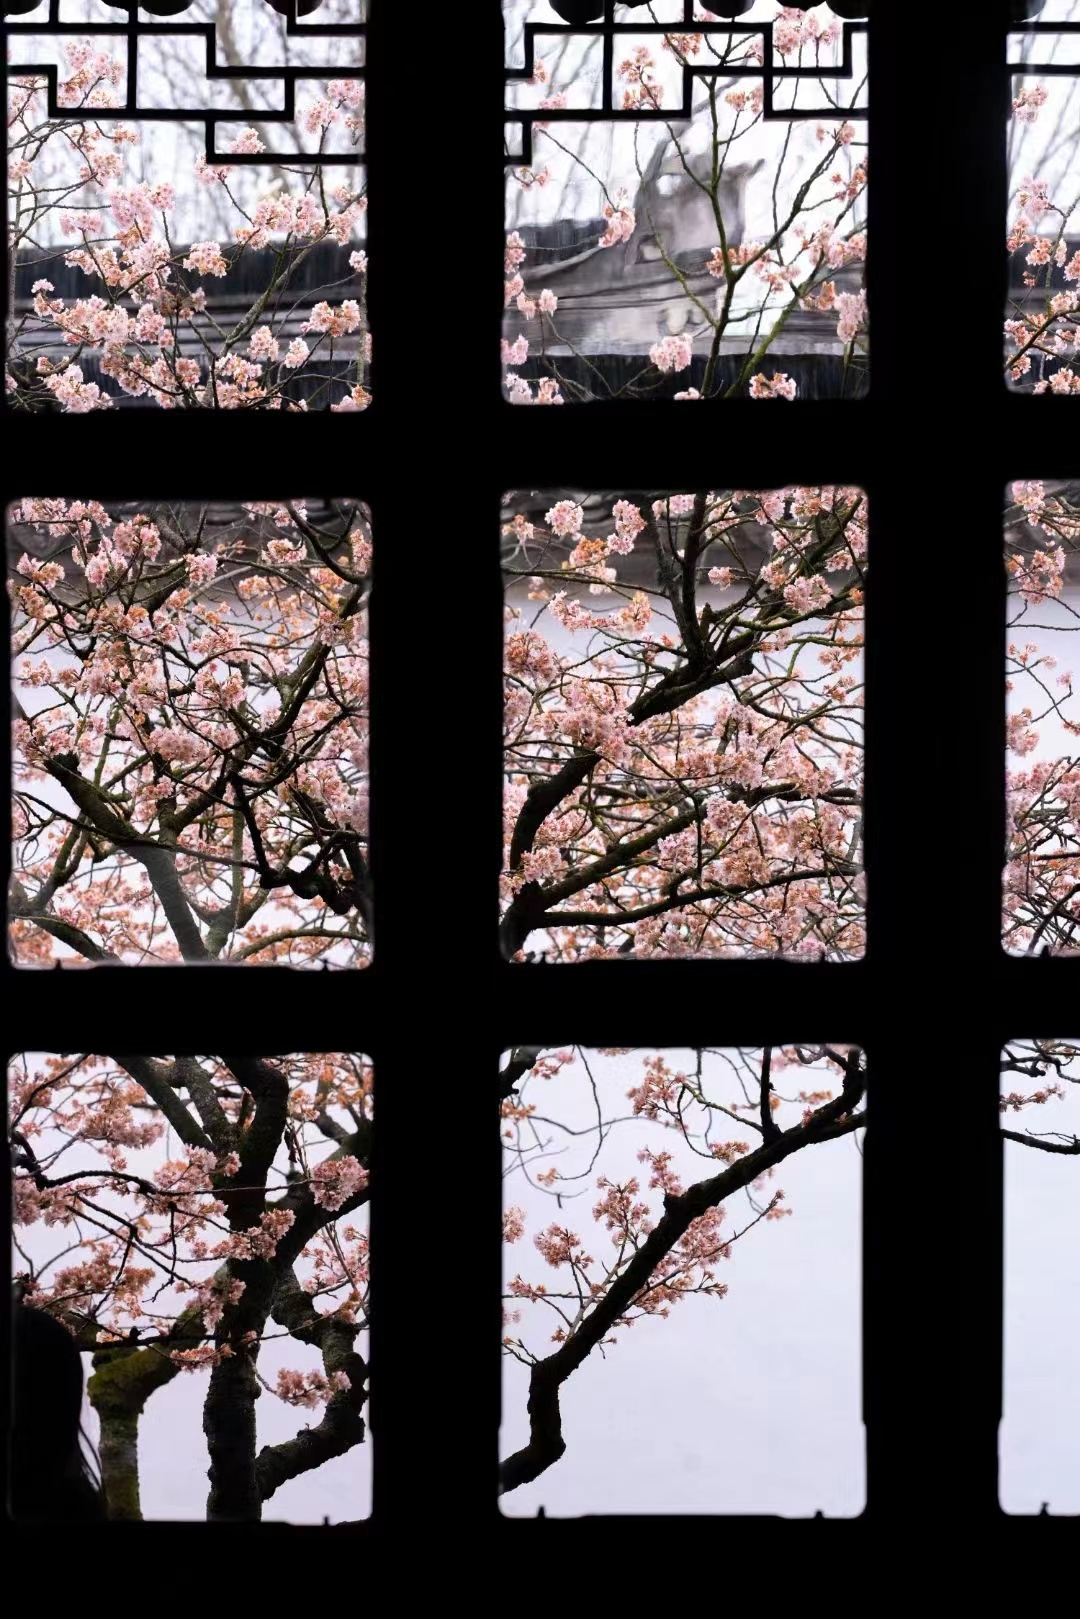
\includegraphics[width=.5\textwidth,height=.5\textheight,keepaspectratio]{题照拙句.jpg}
\end{center}

\begin{common-format}
\addchtoc{前言}
\chapter*{前言}

此电子版本乃由Ned Walsh于一九九二年春陆续输入。当时他是美国Columbia大学的博士班学生。他断断续续地学习了十年的中文,其博士论文的主题将是关于北宋时期的词。我于该年春末将全文校正一遍,并稍改Ned的格式。全本共有三百又二十首诗,原由蘅塘退士选辑,分为六卷。以下目录中,右端列的是诗的编号。

——单维彰 1992-7-5

标点、国标版制作 ——方舟子

用\LaTeX 排版,部分不明确的字结合手写输入和网络资源明确电脑输入,然后参考汉典给出基本字义。——万泽 2014-10。

更新\LaTeX 注音排版。增补几首常背诗篇(;>),一并音注。 ——Kevin(凯文) 2024-5。

%这里空一行。

\end{common-format}


\addchtoc{目录}
\setcounter{tocdepth}{3}
\tableofcontents

% \begin{common-format}
\mainmatter

\part{五言古诗}

\chapter{汉乐府:白头吟}
\begin{poemzh}{汉乐府}{白头吟}
皑如山上雪,皎若云间月。\\
闻君有两意,故来相决绝。\\
今日斗酒会,明旦沟水头。\\
躞蹀御沟上,沟水东西流。\\
凄凄复凄凄,嫁娶不须啼。\\
愿得一心人,白头不相离。\\
竹竿何嫋嫋,鱼尾何簁簁!\\
男儿重意气,何用钱刀为!\\
\end{poemzh}

\chapter{佚名:古诗十九首之迢迢牵牛星}
\begin{poemzh}{东汉·佚名}{古诗十九首之迢迢牵牛星}
迢迢牵牛星,皎皎河汉女。\\
纤纤擢素手,札札弄机杼。\\ 
终日不成章,泣涕零如雨。\\
河汉清且浅,相去复几许!\\ 
盈盈一水间,脉脉不得语。\\
\end{poemzh}

\chapter{张九龄:感遇四首之一}
\begin{poemzh}{张九龄}{感遇四首之一}
孤鸿海上来,池潢不敢顾。\\
侧见双翠鸟,巢在三珠树。\\
矫矫珍木巅,得无金丸惧。\\
美服患人指,高明逼神恶。\\
今我游冥冥,弋者何所慕。\\ 
\end{poemzh}

\chapter{张九龄:感遇四首之二}
\begin{poemzh}{张九龄}{感遇四首之二}
兰叶春葳蕤,桂华秋皎洁。\\
欣欣此生意,自尔为佳节。\\
谁知林栖者,闻风坐相悦。\\
草木有本心,何求美人折?\\ 
\end{poemzh}
  


\chapter{张九龄:感遇四首之三}
\begin{poemzh}{张九龄}{感遇四首之三}
幽人归独卧,滞虑洗孤清。\\
持此谢高鸟,因之传远情。\\
日夕怀空意,人谁感至精?\\
飞沈理自隔,何所慰吾诚?\\ 
\end{poemzh}

\chapter{张九龄:感遇四首之四}
\begin{poemzh}{张九龄}{感遇四首之四}
江南有丹橘,经冬犹绿林。\\
岂伊地气暖,自有岁寒心。\\
可以荐嘉客,奈何阻重深!\\
运命惟所遇,循环不可寻。\\
徒言树桃李,此木岂无阴?\\ 
\end{poemzh}

\chapter{李白:下终南山过斛斯山人宿置酒}
\begin{poemzh}{李白}{下终南山过斛斯山人宿置酒}
暮从碧山下,山月随人归,\\
却顾所来径,苍苍横翠微。\\
相携及田家,童稚开荆扉。\\
绿竹入幽径,青萝拂行衣。\\
欢言得所憩,美酒聊共挥。\\
长歌吟松风,曲尽河星稀。\\
我醉君复乐,陶然共忘机。\\ 
\end{poemzh}

\chapter{李白:月下独酌}
\begin{poemzh}{李白}{月下独酌}
花间一壶酒,独酌无相亲。\\
举杯邀明月,对影成三人。\\
月既不解饮,影徒随我身。\\
暂伴月将影,行乐须及春。\\
我歌月徘徊,我舞影零乱。\\
醒时同交欢,醉后各分散。\\
永结无情游,相期邈云汉。\\ 
\end{poemzh}

\chapter{李白:春思}
\begin{poemzh}{李白}{春思}
燕草如碧丝,秦桑低绿枝。\\
当君怀归日,是妾断肠时。\\
春风不相识,何事入罗帏?\\ 
\end{poemzh}

\chapter{杜甫:望岳}
\begin{poemzh}{杜甫}{望岳}
岱宗夫如何,齐鲁青未了。\\
造化钟神秀,阴阳割昏晓。\\
\xpinyin{汤}{dang4}胸生层云,决眦入归鸟,\\
会当凌绝顶,一览众山小。\\ 
\end{poemzh}


\chapter{杜甫:赠卫八处士}
\begin{poemzh}{杜甫}{赠卫八处士}
人生不相见,动如参与商。\\
今夕复何夕,共此灯烛光。\\
少壮能几时,鬓发各已苍。\\
访旧半为鬼,惊呼热中肠。\\
焉知二十载,重上君子堂。\\
昔别君未婚,儿女忽成行。\\
怡然敬父执,问我来何方。\\
问答乃未已,驱儿罗酒浆。\\
夜雨剪春韭,新炊间黄粱。\\
主称会面难,一举累十觞。\\
十觞亦不醉,感子故意长。\\
明日隔山岳,世事两茫茫。\\ 
\end{poemzh}


\chapter{杜甫:佳人}
\begin{poemzh}{杜甫}{佳人}
绝代有佳人,幽居在空谷。\\
自云良家子,零落依草木。\\
关中昔丧乱,兄弟遭杀戮。\\
官高何足论,不得收骨肉。\\
世情恶衰歇,万事随转烛。\\
夫婿轻薄儿,新人美如玉。\\
合昏尚知时,鸳鸯不独宿。\\
但见新人笑,那闻旧人哭!\\
在山泉水清,出山泉水浊。\\
侍婢卖珠回,牵萝补茅屋。\\
摘花不插发,采柏动盈掬。\\
天寒翠袖薄,日暮倚修竹。\\ 
\end{poemzh}

\chapter{杜甫:梦李白二首之一}
\begin{poemzh}{杜甫}{梦李白二首之一}
死别已吞声,生别常恻恻。\\
江南瘴疠地,逐客无消息。\\
故人入我梦,明我长相忆。\\
君今在罗网,何以有羽翼?\\
恐非平生魂,路远不可测。\\
魂来枫林青,魂返关塞黑。\\
落月满屋梁,犹疑照颜色。\\
水深波浪阔,无使蛟龙得。\\ 
\end{poemzh}



\chapter{杜甫:梦李白二首之二}
\begin{poemzh}{杜甫}{梦李白二首之二}
浮云终日行,游子久不至。\\
三夜频梦君,情亲见君意。\\
告归常局促,苦道来不易。\\
江湖多风波,舟楫恐失坠。\\
出门搔白首,若负平生志。\\
冠盖满京华,斯人独憔悴。\\
孰云网恢恢,将老身反累。\\
千秋万岁名,寂寞身后事。\\
\end{poemzh}

\chapter{王维:送别}
\begin{poemzh}{王维}{送别}
下马饮君酒,问君何所之。\\
君言不得意,归卧南山陲。\\
但去莫复闻,白云无尽时。\\ 
\end{poemzh}

\chapter{王维:送綦毋潜落第还乡}
\begin{poemzh}{王维}{送綦毋潜落第还乡}
圣代无隐者,英灵尽来归。\\
遂令东山客,不得顾采薇。\\
既至金门远,孰云吾道非?\\
江淮度寒食,京洛缝春衣。\\
置酒长安道,同心与我违。\\
行当浮桂棹,未几拂荆扉。\\
远树带行客,孤城当落晖。\\
吾谋适不用,勿谓知音稀。\\ 
\end{poemzh}

\chapter{王维:青溪}
\begin{poemzh}{王维}{青溪}
言入黄花川,每逐青溪水。\\
随山将万转,趣途无百里。\\
声喧乱石中,色静深松里。\\
漾漾泛菱荇,澄澄映葭苇。\\
我心素已闲,清川澹如此。\\
请留盘石上,垂钓将已矣。\\ 
\end{poemzh}

\chapter{王维:渭川田家}
\begin{poemzh}{王维}{渭川田家}
斜光照墟落,穷巷牛羊归。\\
野老念牧童,倚杖候荆扉。\\
雉雊麦苗秀,蚕眠桑叶稀。\\
田夫荷锄立,相见语依依。\\
即此羡闲逸,怅然吟式微。\\ 
\end{poemzh}


\begin{itemize}
\item 雊(gòu):野鸡叫。
\end{itemize}

\chapter{王维:西施咏}
\begin{poemzh}{王维}{西施咏}
艳色天下重,西施宁久微。\\
朝为越溪女,暮作吴宫妃。\\
贱日岂殊众,贵来方悟稀。\\
邀人傅脂粉,不自著罗衣。\\
君宠益娇态,君怜无是非。\\
当时浣纱伴,莫得同车归。\\
持谢邻家子,效颦安可希!\\ 
\end{poemzh}

\chapter{孟浩然:秋登兰山寄张五}
\begin{poemzh}{孟浩然}{秋登兰山寄张五}
北山白云里,隐者自怡悦。\\
相望始登高,心随雁飞灭。\\
愁因薄暮起,兴是清秋发。\\
时见归村人,沙行渡头歇。\\
天边树若荠,江畔洲如月。\\
何当载酒来,共醉重阳节。\\ 
\end{poemzh}

\chapter{孟浩然:夏日南亭怀辛大}
\begin{poemzh}{孟浩然}{夏日南亭怀辛大}
山光忽西落,池月渐东上。\\
散发乘夜凉,开轩卧闲敞。\\
荷风送香气,竹露滴清响。\\
欲取鸣琴弹,恨无知音赏。\\
感此怀故人,中宵劳梦想。\\ 
\end{poemzh}

\chapter{孟浩然:宿业师山房待丁大不至}
\begin{poemzh}{孟浩然}{宿业师山房待丁大不至}
夕阳度西岭,群壑倏已暝。\\
松月生夜凉,风泉满清听。\\
樵人归欲尽,烟鸟栖初定。\\
之子期宿来,孤琴候萝径。\\ 
\end{poemzh}

\chapter{王昌龄:同从弟南斋玩月忆山阴崔少府}
\begin{poemzh}{王昌龄}{同从弟南斋玩月忆山阴崔少府}
高卧南斋时,开帷月初吐。\\
清辉淡水木,演漾在窗户。\\
苒苒几盈虚,澄澄变今古。\\
美人清江畔,是夜越吟苦。\\
千里其如何,微风吹兰杜。\\ 
\end{poemzh}

\chapter{邱为:寻西山隐者不遇}
\begin{poemzh}{邱为}{寻西山隐者不遇}
绝顶一茅茨,直上三十里。\\
扣关无僮仆,窥室惟案几。\\
若非巾柴车,应是钓秋水。\\
差池不相见,黾勉空仰止。\\
草色新雨中,松声晚窗里。\\
及兹契幽绝,自足荡心耳。\\
虽无宾主意,颇得清净理。\\
兴尽方下山,何必待之子。\\ 
\end{poemzh}

\chapter{綦毋潜:春泛若耶溪}
\begin{poemzh}{綦毋潜}{春泛若耶溪}
幽意无断绝,此去随所偶。\\
晚风吹行舟,花路入溪口。\\
际夜转西壑,隔山望南斗。\\
潭烟飞溶溶,林月低向后。\\
生事且弥漫,愿为持竿叟。\\ 
\end{poemzh}

\chapter{常建:宿王昌龄隐居}
\begin{poemzh}{常建}{宿王昌龄隐居}
清溪深不测,隐处唯孤云。\\
松际露微月,清光犹为君。\\
茅亭宿花影,药院滋苔纹。\\
余亦谢时去,西山鸾鹤群。\\ 
\end{poemzh}

\chapter{岑参:与高适薛据登慈恩寺浮图}
\begin{poemzh}{岑参}{与高适薛据登慈恩寺浮图}
塔势如涌出,孤高耸天宫。\\
登临出世界,磴道盘虚空。\\
突兀压神州,峥嵘如鬼工。\\
四角碍白日,七层摩苍穹。\\
下窥指高鸟,俯听闻惊风。\\
连山若波涛,奔凑如朝东。\\
青槐夹驰道,宫馆何玲珑!\\
秋色从西来,苍然满关中。\\
五陵北原上,万古青蒙蒙。\\
净理了可悟,胜因夙所宗。\\
誓将挂冠去,觉道资无穷。\\ 
\end{poemzh}

\chapter{元结:贼退示官吏并序}
癸卯岁,西原贼入道州,焚烧杀掠,几尽而去。明年,贼又攻永州,破邵,不犯此州边鄙而退,岂力能制敌欤?盖蒙其伤怜而已!诸史何为忍苦征敛!故作诗一篇以示官吏。

\begin{poemzh}{元结}{贼退示官吏并序}
昔岁逢太平,山林二十年。\\
泉源在庭户,洞壑当门前。\\
井税有常期,日晏犹得眠。\\
忽然遭时变,数岁亲戎旃。\\
今来典斯郡,山夷又纷然。\\
城小贼不屠,人贫伤可怜。\\
是以陷邻境,此州独见全。\\
使臣将王命,岂不如贼焉!\\
令彼征敛者,迫之如火煎。\\
谁能绝人命,以作时世贤。\\
思欲委符节,引竿自刺船。\\
将家就鱼麦,归老江湖边。\\ 
\end{poemzh}


\chapter{韦应物:郡斋雨中与诸文士燕集}
\begin{poemzh}{韦应物}{郡斋雨中与诸文士燕集}
兵卫森画戟,宴寝凝清香。\\
海上风雨至,逍遥池阁凉。\\
烦疴近消散,嘉宾复满堂。\\
自惭居处崇,未睹斯民康。\\
理会是非遣,性达形迹忘。\\
鲜肥属时禁,蔬果幸见尝。\\
俯饮一杯酒,仰聆金玉章。\\
神欢体自轻,意欲凌风翔。\\
吴中盛文史,群彦今汪洋。\\
方知大蕃地,岂曰财赋强。\\ 
\end{poemzh}

\chapter{韦应物:初发扬子寄元大校书}
\begin{poemzh}{韦应物}{初发扬子寄元大校书}
凄凄去亲爱,泛泛入烟雾。\\
归棹洛阳人,残钟广陵树。\\
今朝为此别,何处还相遇。\\
世事波上舟,沿洄安得住。\\ 
\end{poemzh}

\chapter{韦应物:寄全椒山中道士}
\begin{poemzh}{韦应物}{寄全椒山中道士}
今朝郡斋冷,忽念山中客。\\
涧底束荆薪,归来煮白石。\\
欲持一瓢酒,远慰风雨夕。\\
落叶满空山,何处寻行迹。\\ 
\end{poemzh}

\chapter{韦应物:长安遇冯著}
\begin{poemzh}{韦应物}{长安遇冯著}
客从东方来,衣上灞陵雨。\\
问客何为来,采山因买斧。\\
冥冥花正开,扬扬燕新乳。\\
昨别今已春,鬓丝生几缕。\\ 
\end{poemzh}

\chapter{韦应物:夕次盱眙县}
\begin{poemzh}{韦应物}{夕次盱眙县}
落帆逗淮镇,停舫临孤驿。\\
浩浩风起波,冥冥日沈夕。\\
人归山郭暗,雁下芦洲白。\\
独夜忆秦关,听钟未眠客。\\ 
\end{poemzh}

\chapter{韦应物:东郊}
\begin{poemzh}{韦应物}{东郊}
吏舍局终年,出郊旷清曙。\\
杨柳散和风,青山澹吾虑。\\
依丛适自憩,缘涧还复去。\\
微雨霭芳原,春鸠鸣何处?\\
乐幽心屡止,遵事迹犹遽。\\
终罢斯结庐,慕陶真可庶。\\ 
\end{poemzh}

\chapter{韦应物:送杨氏女}
\begin{poemzh}{韦应物}{送杨氏女}
永日方戚戚,出行复悠悠。\\
女子今有行,大江溯轻舟。\\
尔辈苦无恃,抚念益慈柔。\\
幼为长所育,两别泣不休。\\
对此结中肠,义往难复留!\\
自小阙内训,事姑贻我忧。\\
赖兹托令门,仁恤庶无尤。\\
贫俭诚所尚,资从岂待周?\\
孝恭遵妇道,容止顺其猷。\\
别离在今晨,见尔当何秋。\\
居闲始自遣,临感忽难收。\\
归来视幼女,零泪缘缨流。\\ 
\end{poemzh}

\chapter{柳宗元:晨诣超师院读禅经}
\begin{poemzh}{柳宗元}{晨诣超师院读禅经}
汲井漱寒齿,清心拂尘服。\\
闲持贝叶书,步出东斋读。\\
真源了无取,忘迹世所逐。\\
遗言冀可冥,缮性何由熟?\\
道人庭宇静,苔色连深竹。\\
日出雾露馀,青松如膏沐。\\
澹然离言说,悟悦心自足。\\ 
\end{poemzh}

\chapter{柳宗元:溪居}
\begin{poemzh}{柳宗元}{溪居}
久为簪组累,幸此南夷谪。\\
闲依农圃邻,偶似山林客。\\
晓耕翻露草,夜榜响溪石。\\
来往不逢人,长歌楚天碧。\\ 
\end{poemzh}

\chapter{王昌龄:塞上曲}
\begin{poemzh}{王昌龄}{塞上曲}
蝉鸣空桑林,八月萧关道。\\
出塞复入塞,处处黄芦草。\\
从来幽并客,皆向沙场老。\\
莫学游侠儿,矜夸紫骝好。\\ 
\end{poemzh}


\chapter{王昌龄:塞下曲}
\begin{poemzh}{王昌龄}{塞下曲}
饮马渡秋水,水寒风似刀。\\
平沙日未没,黯黯见临洮。\\
昔日长城战,咸言意气高。\\
黄尘足今古,白骨乱蓬蒿。\\ 
\end{poemzh}

\chapter{李白:关山月}
\begin{poemzh}{李白}{关山月}
明月出天山,苍茫云海间。\\
长风几万里,吹度玉门关。\\
汉下白登道,胡窥青海湾。\\
由来征战地,不见有人还。\\
戍客望边色,思归多苦颜。\\
高楼当此夜,叹息未应闲。\\ 
\end{poemzh}

\chapter{李白:子夜四时歌:春歌}
\begin{poemzh}{李白:子夜四时歌}{春歌}
秦地罗敷女,采桑绿水边。\\
素手青条上,红妆白日鲜。\\
蚕饥妾欲去,五马莫留连。\\ 
\end{poemzh}

\chapter{李白:子夜四时歌:夏歌}
\begin{poemzh}{李白:子夜四时歌}{夏歌}
镜湖三百里,菡萏发荷花。\\
五月西施采,人看隘若耶。\\
回舟不待月,归去越王家。\\ 
\end{poemzh}

\chapter{李白:子夜四时歌:秋歌}
\begin{poemzh}{李白:子夜四时歌}{秋歌}
长安一片月,万户捣衣声。\\
秋风吹不尽,总是玉关情。\\
何日平胡虏,良人罢远征?\\ 
\end{poemzh}

\chapter{李白:子夜四时歌:冬歌}
\begin{poemzh}{李白:子夜四时歌}{冬歌}
明朝驿使发,一夜絮征袍。\\
素手抽针冷,那堪把剪刀。\\
裁缝寄远道,几日到临洮?\\ 
\end{poemzh}

\chapter{李白:长干行}
\begin{poemzh}{李白}{长干行}
妾发初覆额,折花门前剧。\\
郎骑竹马来,绕床弄青梅。\\
同居长干里,两小无嫌猜。\\
十四为君妇,羞颜未尝开。\\
低头向暗壁,千唤不一回。\\
十五始展眉,愿同尘与灰。\\
常存抱柱信,岂上望夫台!\\
十六君远行,瞿塘滟预堆。\\
五月不可触,猿鸣天上哀。\\
门前迟行迹,一一生绿苔。\\
苔深不能扫,落叶秋风早。\\
八月蝴蝶来,双飞西园草。\\
感此伤妾心,坐愁红颜老。\\
早晚下三巴,预将书报家。\\
相迎不道远,直至长风沙。\\ 
\end{poemzh}

\chapter{孟郊:烈女操}
\begin{poemzh}{孟郊}{烈女操}
梧桐相待老,鸳鸯会双死。\\
贞妇贵殉夫,舍生亦如此。\\
波澜誓不起,妾心井中水。\\ 
\end{poemzh}

\chapter{孟郊:游子吟}
\begin{poemzh}{孟郊}{游子吟}
慈母手中线,游子身上衣。\\
临行密密缝,意恐迟迟归。\\
谁言寸草心,报得三春辉?\\ 
\end{poemzh}

\chapter{陈子昂:登幽州台歌}
\begin{poemzh}{陈子昂}{登幽州台歌}
前不见古人,后不见来者。\\
念天地之悠悠,独怆然而涕下!\\ 
\end{poemzh}

\chapter*{凯文:无题}
\begin{poemzh}{现代·凯文}{无题}
故事或旧闻,体态已察觉。\\
儿时少顷梦\footnote[1]{小时候看到、体察的世界,是长大后思维基本模型的原型和基础。},云龙舞腾挪。\\
虚伪多假事,情趣难捉摸。\\
觅觅金钞\xpinyin{卷}{juan4},一一粪土说。\\
求仙也问道,鬼神无通灵。\\
何来证教义,家规毋须多。\\
天\xpinyin{地}{di4}犹橐龠,万物自开合。\\
汝心求正主,琴瑟待声\xpinyin{和}{he4}。\\
\end{poemzh}

\part{七言古诗}

\chapter{王勃:滕王阁序并诗}

豫章故郡,洪都新府。星分翼轸,地接衡庐。襟三江而带五湖,控蛮荆而引瓯越。物华天宝,龙光射牛斗之墟;人杰地灵,徐孺下陈蕃之榻。雄州雾列,俊采星驰。台隍枕夷夏之交,宾主尽东南之美。都督阎公之雅望,棨戟遥临;宇文新州之懿范,襜帷暂驻。十旬休假,胜友如云;千里逢迎,高朋满座。腾蛟起凤,孟学士之词宗;紫电青霜,王将军之武库。家君作宰,路出名区;童子何知,躬逢胜饯。

时维九月,序属三秋。潦水尽而寒潭清,烟光凝而暮山紫。俨骖騑于上路,访风景于崇阿。临帝子之长洲,得天人之旧馆。层峦耸翠,上出重霄;飞阁流丹,下临无地。鹤汀凫渚,穷岛屿之萦回;桂殿兰宫,即冈峦之体势。

披绣闼,俯雕甍,山原旷其盈视,川泽纡其骇瞩。闾阎扑地,钟鸣鼎食之家;舸舰弥津,青雀黄龙之舳。云销雨霁,彩彻区明。落霞与孤鹜齐飞,秋水共长天一色。渔舟唱晚,响穷彭蠡之滨;雁阵惊寒,声断衡阳之浦。

遥襟甫畅,逸兴遄飞。爽籁发而清风生,纤歌凝而白云遏。睢园绿竹,气凌彭泽之樽;邺水朱华,光照临川之笔。四美具,二难并。穷睇眄于中天,极娱游于暇日。天高地迥,觉宇宙之无穷;兴尽悲来,识盈虚之有数。望长安于日下,目吴会于云间。地势极而南溟深,天柱高而北辰远。关山难越,谁悲失路之人;萍水相逢,尽是他乡之客。怀帝阍而不见,奉宣室以何年?

嗟乎!时运不齐,命途多舛。冯唐易老,李广难封。屈贾谊于长沙,非无圣主;窜梁鸿于海曲,岂乏明时?所赖君子见机,达人知命。老当益壮,宁移白首之心?穷且益坚,不坠青云之志。酌贪泉而觉爽,处涸辙以犹欢。北海虽赊,扶摇可接;东隅已逝,桑榆非晚。孟尝高洁,空余报国之情;阮籍猖狂,岂效穷途之哭!

勃,三尺微命,一介书生。无路请缨,等终军之弱冠;有怀投笔,慕宗悫之长风。舍簪笏于百龄,奉晨昏于万里。非谢家之宝树,接孟氏之芳邻。他日趋庭,叨陪鲤对;今兹捧袂,喜托龙门。杨意不逢,抚凌云而自惜;钟期既遇,奏流水以何惭?

呜乎!胜地不常,盛筵难再;兰亭已矣,梓泽丘墟。临别赠言,幸承恩于伟饯;登高作赋,是所望于群公。敢竭鄙怀,恭疏短引;一言均赋,四韵俱成。请洒潘江,各倾陆海云尔!

\begin{poemzh}{王勃}{滕王阁}
滕王高阁临江渚,佩玉鸣鸾罢歌舞。\\
画栋朝飞南浦云,珠帘暮卷西山雨。\\
闲云潭影日悠悠,物换星移几度秋。\\
阁中帝子今何在?槛外长江空自流。\\
\end{poemzh}

\chapter{李颀:古意}
\begin{poemzh}{李颀}{古意}
男儿事长征,少小幽燕客。\\
赌胜马蹄下,由来轻七尺。\\
杀人莫敢前,须如猬毛磔。\\
黄云陇底白雪飞,未得报恩不能归。\\
辽东小妇年十五,惯弹琵琶解歌舞。\\
今为羌笛出塞声,使我三军泪如雨!\\ 
\end{poemzh}

\chapter{李颀:送陈章甫}
\begin{poemzh}{李颀}{送陈章甫}
四月南风大麦黄,枣花未落桐叶长。\\
青山朝别暮还见,嘶马出门思故乡。\\
陈侯立身何坦荡,虬须虎眉仍大颡。\\
腹中贮书一万卷,不肯低头在草莽。\\
东门酤酒饮我曹,心轻万事皆鸿毛。\\
醉卧不知白日暮,有时空望孤云高。\\
长河浪头连天黑,津口停舟渡不得。\\
郑国游人未及家,洛阳行子空叹息。\\
闻道故林相识多,罢官昨日今如何?\\ 
\end{poemzh}

\chapter{李颀:琴歌}
\begin{poemzh}{李颀}{琴歌}
主人有酒欢今夕,请奏鸣琴广陵客。\\
月照城头乌半飞,霜凄万树风入衣。\\
铜炉华烛烛增辉,初弹渌水后楚妃。\\
一声已动物皆静,四座无言星欲稀。\\
清淮奉使千馀里,敢告云山从此始?\\ 
\end{poemzh}

\chapter{李颀:听董大弹胡笳声兼寄语弄房给事}
\begin{poemzh}{李颀}{听董大弹胡笳声兼寄语弄房给事}
蔡女昔造胡笳声,一弹一十有八拍。\\
胡人落泪沾边草,汉使断肠对归客。\\
古戍苍苍烽火寒,大荒沈沈飞雪白。\\
先拂声弦后角羽,四郊秋叶惊摵摵。\\
董夫子,通神明,深山窃听来妖精。\\
言迟更速皆应手,将往复旋如有情。\\
空山百鸟散还合,万里浮云阴且晴。\\
嘶酸雏雁失群夜,断绝胡儿恋母声。\\
川为静其波,鸟亦罢其鸣。\\
乌孙部落家乡远,逻娑沙尘哀怨生。\\
幽音变调忽飘洒,长风吹林雨堕瓦。\\
迸泉飒飒飞木末,野鹿呦呦走堂下。\\
长安城连东掖垣,凤凰池对青琐门。\\
高才脱略名与利,日夕望君抱琴至。\\ 
\end{poemzh}

\begin{itemize}
\item 摵(sè):古同“槭”,树枝光秃,叶凋落的样子。
\end{itemize}

\chapter{李颀:听安万善吹筚篥歌}
\begin{poemzh}{李颀}{听安万善吹筚篥歌}
南山截竹为筚篥,此乐本自龟兹出。\\
流传汉地曲转奇,凉州胡人为我吹。\\
傍邻闻者多叹息,远客思乡皆泪垂。\\
世人解听不解赏,长飙风中自来往。\\
枯桑老柏寒飕飗,九雏鸣凤乱啾啾。\\
龙吟虎啸一时发,万籁百泉相与秋。\\
忽然更作渔阳掺,黄云萧条白日暗。\\
变调如闻杨柳春,上林繁花照眼新。\\
岁夜高堂列明烛,美酒一杯声一曲。\\ 
\end{poemzh}

\begin{itemize}
\item 飗(liú):微风吹动的样子。
\end{itemize}

\chapter{孟浩然:夜归鹿门山歌}
\begin{poemzh}{孟浩然}{夜归鹿门山歌}
山寺钟鸣昼已昏,渔梁渡头争渡喧。\\
人随沙路向江村,余亦乘舟归鹿门。\\
鹿门月照开烟树,忽到庞公栖隐处。\\
岩扉松径长寂寥,惟有幽人自来去。\\ 
\end{poemzh}

\chapter{李白:庐山谣寄卢侍御虚舟}
\begin{poemzh}{李白}{庐山谣寄卢侍御虚舟}
我本楚狂人,凤歌笑孔丘。\\
手持绿玉杖,朝别黄鹤楼。\\
五岳寻仙不辞远,一生好入名山游。\\
庐山秀出南斗傍,屏风九叠云锦张。\\
影落明湖青黛光,金阙前开二峰长。\\
银河倒挂三石梁,香炉瀑布遥相望。\\
回崖沓障凌苍苍。\\
翠影红霞映朝日,鸟飞不到吴天长。\\
登高壮观天地间,大江茫茫去不黄。\\
黄云万里动风色,白波九道流雪山。\\
好为庐山谣,兴因庐山发。\\
闲窥石镜清我心,谢公行处苍苔没。\\
早服还丹无世情,琴心三叠道初成。\\
遥见仙人彩云里,手把芙蓉朝玉京。\\
先期汗漫九垓上,愿接卢敖游太清。\\ 
\end{poemzh}

\chapter{李白:梦游天姥吟留别}
\begin{poemzh}{李白}{梦游天姥吟留别}
海客谈瀛洲,烟涛微茫信难求。\\
越人语天姥,云霓明灭或可睹。\\
天姥连天向天横,势拔五岳掩赤城。\\
天台四万八千丈,对此欲倒东南倾。\\
我欲因之梦吴越,一夜飞渡镜湖月。\\
湖月照我影,送我至剡溪。\\
谢公宿处今尚在,渌水荡漾清猿啼。\\
脚著谢公屐,身登青云梯。\\
半壁见海日,空中闻天鸡。\\
千岩万壑路不定,迷花倚石忽已暝。\\
熊咆龙吟殷岩泉,栗深林兮惊层巅。\\
云青青兮欲雨,水澹澹兮生烟。\\
裂缺霹雳,丘峦崩摧。\\
洞天石扇,訇然中开。\\
青冥浩荡不见底,日月照耀金银台。\\
霓为衣兮风为马,云之君兮纷纷而来下。\\
虎鼓瑟兮鸾回车,仙之人兮列如麻。\\
忽魂悸以魄动,恍惊起而长嗟。\\
惟觉时之枕席,失向来之烟霞。\\
世间行乐亦如此,古来万事东流水。\\
别君去兮何时还?且放白鹿青崖间。\\
须行即骑访名山。\\
安能摧眉折腰事权贵,使我不得开心颜!\\ 
\end{poemzh}

\chapter{李白:金陵酒肆留别}
\begin{poemzh}{李白}{金陵酒肆留别}
风吹柳花满店香,吴姬压酒唤客尝。\\
金陵子弟来相送,欲行不行各尽觞。\\
请君试问东流水,别意与之谁短长?\\ 
\end{poemzh}

\chapter{李白:宣州谢朓楼饯别校书叔云}
\begin{poemzh}{李白}{宣州谢朓楼饯别校书叔云}
弃我去者,昨日之日不可留。\\
乱我心者,今日之日多烦忧!\\
长风万里送秋雁,对此可以酣高楼。\\
蓬莱文章建安骨,中间小谢又清发。\\
俱怀逸兴壮思飞,欲上青天览明月。\\
抽刀断水水更流,举杯销愁愁更愁。\\
人生在世不称意,明朝散发弄扁舟。\\ 
\end{poemzh}

\begin{itemize}
\item 朓(tiǎo)。
\end{itemize}


\chapter{岑参:走马川行奉送封大夫出师西征}
\begin{poemzh}{岑参}{走马川行奉送封大夫出师西征}
君不见走马川行雪海边,平沙莽莽黄入天。\\
轮台九月风夜吼,一川碎石大如斗。\\
随风满地石乱走,匈奴草黄马正肥。\\
金山西见烟尘飞,汉家大将西出师。\\
将军金甲夜不脱,半夜军行戈相拨。\\
风头如刀面如割,马毛带雪汗气蒸。\\
五花连钱旋作冰,幕中草檄砚水凝。\\
虏骑闻之应胆慑,料知短兵不敢接。\\
车师西门伫献捷!\\ 
\end{poemzh}

\chapter{岑参:轮台歌奉送封大夫出师西征}
\begin{poemzh}{岑参}{轮台歌奉送封大夫出师西征}
轮台城头夜吹角,轮台城北旄头落。\\
羽书昨夜过渠黎,单于已在金山西。\\
戍楼西望烟尘黑,汉兵屯在轮台北。\\
上将拥旄西出征,平明吹笛大军行。\\
四边伐鼓雪海涌,三军大呼阴山动。\\
虏塞兵气连云屯,战场白骨缠草根。\\
剑河风急雪片阔,沙口石冻马蹄脱。\\
亚相勤王甘苦辛,誓将报主静边尘。\\
古来青史谁不见,今见功名胜古人。\\ 
\end{poemzh}

\chapter{岑参:白雪歌送武判官归京}
\begin{poemzh}{岑参}{白雪歌送武判官归京}
北风卷地白草折,胡天八月即飞雪。\\
忽如一夜春风来,千树万树梨花开。\\
散入珠帘湿罗幕,狐裘不暖锦衾薄。\\
将军角弓不得控,都护铁衣冷犹著。\\
瀚海阑干百丈冰,愁云黪淡万里凝。\\
中军置酒饮归客,胡琴琵琶与羌笛。\\
纷纷暮雪下辕门,风掣红旗冻不翻。\\
轮台东门送君去,去时雪满天山路。\\
山回路转不见君,雪上空留马行处。\\ 
\end{poemzh}

\chapter{杜甫:韦讽录事宅观曹将军画马图}
\begin{poemzh}{杜甫}{韦讽录事宅观曹将军画马图}
国初以来画鞍马,神妙独数江都王。\\
将军得名三十载,人间又见真乘黄。\\
曾貌先帝照夜白,龙池十日飞霹雳。\\
内府殷红玛瑙盘,婕妤传诏才人索。\\
盘赐将军拜舞归,轻纨细绮相追飞。\\
贵戚权门得笔迹,始觉屏障生光辉。\\
昔日太宗拳毛騧,近时郭家狮子花。\\
今之新图有二马。复令识者久叹嗟。\\
此皆骑战一敌万,缟素漠漠开风沙。\\
其余七匹亦殊绝,迥若寒空杂烟雪。\\
霜蹄蹴踏长楸间,马官厮养森成列。\\
可怜九马争神骏,顾视清高气深稳。\\
借问苦心爱者谁,后有韦讽前支盾。\\
忆昔巡幸新丰宫,翠花拂天来向东。\\
腾骧磊落三万匹,皆与此图筋骨同。\\
自从献宝朝河宗,无复射蛟江水中。\\
君不见,金粟堆前松柏里。龙媒去尽鸟呼风。\\ 
\end{poemzh}

\begin{itemize}
\item 騧(guā):黑嘴的黄马。
\end{itemize}

\chapter{杜甫:丹青引赠曹霸将军}
\begin{poemzh}{杜甫}{丹青引赠曹霸将军}
将军魏武之子孙,于今为庶为青门。\\
英雄割据虽已矣,文采风流今尚存。\\
学书初学卫夫人,但恨无过王右军。\\
丹青不知老将至,富贵于我如浮云。\\
开元之中常引见,承恩数上南熏殿。\\
凌烟功臣少颜色,将军下笔开生面。\\
良相头上进贤冠,猛将腰间大羽箭。\\
褒公鄂公毛发动,英姿飒爽犹酣战。\\
先帝天马玉花骢,画工如山貌不同。\\
是日牵来赤墀下,迥立阊阖生长风。\\
诏谓将军拂绢素,意匠惨淡经营中。\\
斯须九重真龙出,一洗万古凡马空。\\
玉花却在御榻上,榻上庭前屹相向。\\
至尊含笑催赐金,圉人太仆皆惆怅。\\
弟子韩干早入室,亦能画马穷殊相。\\
干惟画肉不画骨,忍使骅骝气凋丧。\\
将军画善盖有神,偶逢佳士亦写真。\\
即今漂泊干戈际,屡貌寻常行路人。\\
涂穷反遭俗眼白,世上未有如公贫。\\
但看古来盛名下,终日坎壈缠其身!\\ 
\end{poemzh}

\begin{itemize}
\item 壈(lǎn):不平,喻不顺利,如“英雄坎壈识天意,失路东归亦何济。”
\end{itemize}

\chapter{杜甫:寄韩谏议}
\begin{poemzh}{杜甫}{寄韩谏议}
今我不乐思岳阳,身欲奋飞病在床。\\
美人娟娟隔秋水,濯足洞庭望八荒。\\
鸿飞冥冥日月白,青枫叶赤天雨霜。\\
玉京群帝集北斗,或骑麒麟翳凤凰。\\
芙蓉旌旗烟雾落,影动倒景摇潇湘。\\
星宫之君醉琼浆,羽人稀少不在旁。\\
似闻昨者赤松子,恐是汉代韩张良。\\
昔随刘氏定长安,帷幄未改神惨伤。\\
国家成败吾岂敢,色难腥腐餐枫香。\\
周南留滞古所惜,南极老人应寿昌。\\
美人胡为隔秋水,焉得置之贡玉堂?\\ 
\end{poemzh}

\chapter{杜甫:古柏行}
\begin{poemzh}{杜甫}{古柏行}
孔明庙前有老柏,柯如青铜根如石。\\
双皮溜雨四十围,黛色参天二千尺。\\
君臣已与时际会,树木犹为人爱惜。\\
云来气接巫峡长,月出寒通雪山白。\\
忆昨路绕锦亭东,先主武侯同閟宫。\\
崔嵬枝干郊原古,窈窕丹青户牖空。\\
落落盘踞虽得地,冥冥孤高多烈风。\\
扶持自是神明力,正直元因造化功。\\
大厦如倾要梁栋,万牛回首丘山重。\\
不露文章世已惊,未辞剪伐谁能送?\\
苦心岂免容蝼蚁?香叶终经宿鸾凤。\\
志士幽人莫怨嗟,古来材大难为用!\\ 
\end{poemzh}

\chapter{杜甫:观公孙大娘弟子舞剑器行并序}
大历二年十月十九日夔府别驾元持宅见临颍李十二娘舞剑器,壮其蔚跂。问其所师,曰:余公孙大娘弟子也。开元三载,余尚童稚,记于郾城观公孙氏舞剑器浑脱。浏漓顿挫,独出冠时。自高头宜春梨园二伎坊内人,洎外供奉,晓是舞者,圣文神武皇帝初,公孙一人而已。玉貌锦衣,况余白首!今兹弟子亦匪盛颜。既辨其由来,知波澜莫二。抚事慷慨,聊为剑器行。昔者吴人张旭善草书书帖,数尝於邺县见公孙大娘舞西河剑器,自此草书长进,豪荡感激。即公孙可知矣!

\begin{poemzh}{杜甫}{观公孙大娘弟子舞剑器行并序}
昔有佳人公孙氏,一舞剑器动四方。\\
观者如山色沮丧,天地为之久低昂。\\
霍如羿射九日落,矫如群帝骖龙翔。\\
来如雷霆收震怒,罢如江海凝清光。\\
绛唇珠袖两寂寞,晚有弟子传芬芳。\\
临颍美人在白帝,妙舞此曲神扬扬。\\
与余问答既有以,感时抚事增惋伤。\\
先帝侍女八千人,公孙剑器初第一。\\
五十年间似反掌,风尘澒洞昏王室。\\
梨园子弟散如烟,女乐馀姿映寒日。\\
金粟堆前木已拱,瞿塘石城草萧瑟。\\
玳筵急管曲复终,乐极哀来月东出。\\
老夫不知其所往,足茧荒山转愁疾。\\ 
\end{poemzh}

\begin{itemize}
\item 澒(hòng):〔澒洞(tóng)〕弥漫无边,如“运清浊之澒洞兮,正重沓而并起。”
\end{itemize}

\chapter{元结:石鱼湖上醉歌并序}
漫叟以公田米酿酒,因休暇,则载酒于湖上,时取一醉;欢醉中,据湖岸,引臂向鱼取酒,使舫载之,遍饮坐者。意疑倚巴丘,酌於君山之上,诸子环洞庭而坐,酒舫泛泛然,触波涛而往来者,乃作歌以长之。

\begin{poemzh}{元结}{石鱼湖上醉歌并序}
石鱼湖,似洞庭,夏水欲满君山青。\\
山为樽,水为沼,酒徒历历坐洲鸟。\\
长风连日作大浪,不能废人运酒舫。\\
我持长瓢坐巴丘,酌饮四座以散愁。\\ 
\end{poemzh}

\chapter{韩愈:山石}
\begin{poemzh}{韩愈}{山石}
山石荦确行径微,黄昏到寺蝙蝠飞。\\
升堂坐阶新雨足,芭蕉叶大栀子肥。\\
僧言古壁佛画好,以火来照所见稀。\\
铺床拂席置羹饭,疏粝亦足饱我饥。\\
夜深静卧百虫绝,清月出岭光入扉。\\
天明独去无道路,出入高下穷烟霏。\\
山红涧碧纷烂漫,时见松枥皆十围。\\
当流赤足蹋涧石,水声激激风吹衣。\\
人生如此自可乐,岂必局束为人鞿!\\
嗟哉吾党二三子,安得至老不更归!\\ 
\end{poemzh}

\begin{itemize}
\item 鞿(jī):牵制;束缚。
\end{itemize}

\chapter{韩愈:八月十五夜赠张功曹}
\begin{poemzh}{韩愈}{八月十五夜赠张功曹}
纤云四卷天无河,清风吹空月舒波。\\
沙平水息声影绝,一杯相属君当歌。\\
君歌声酸辞且苦,不能听终泪如雨。\\
洞庭连天九嶷高,蛟龙出没猩鼯号。\\
十生九死到官所,幽居默默如藏逃。\\
下床畏蛇食畏药,海气湿蛰熏腥臊。\\
昨者州前槌大鼓,嗣皇继圣登夔皋。\\
赦书一日行万里,罪从大辟皆除死。\\
迁者追回流者还,涤瑕荡垢清朝班。\\
州家申名使家抑,坎轲只得移荆蛮。\\
判司卑官不堪说,未免捶楚尘埃间。\\
同时辈流多上道,天路幽险难追攀。\\
君歌且休听我歌,我歌今与君殊科。\\
一年明月今宵多,人生由命非由他。\\
有酒不饮奈明何!\\ 
\end{poemzh}

\chapter{韩愈:谒衡岳庙遂宿岳寺题门楼}
\begin{poemzh}{韩愈}{谒衡岳庙遂宿岳寺题门楼}
五岳祭秩皆三公,四方环镇嵩当中。\\
火维地荒足妖怪,天假神柄专其雄。\\
喷云泄雾藏半腹,虽有绝顶谁能穷?\\
我来正逢秋雨节,阴气晦昧无清风。\\
潜心默祷若有应,岂非正直能感通!\\
须臾静扫众峰出,仰见突兀撑青空。\\
紫盖连延接天柱,石廪腾掷堆祝融。\\
森然魄动下马拜,松柏一迳趋灵宫。\\
纷墙丹柱动光彩,鬼物图画填青红。\\
升阶伛偻荐脯酒,欲以菲薄明其衷。\\
庙内老人识神意,睢盱侦伺能鞠躬。\\
手持杯珓导我掷,云此最吉馀难同。\\
窜逐蛮荒幸不死,衣食才足甘长终。\\
侯王将相望久绝,神纵欲福难为功!\\
夜投佛寺上高阁,星月掩映云曈昽。\\
猿鸣钟动不知曙,杲杲寒日生于东。\\ 
\end{poemzh}

\begin{itemize}
\item 珓(jiào):〔杯珓〕占卜的用具,多用两个蚌壳或像蚌壳的竹、木片做成,掷在地上,看它的俯仰,以此占卜吉凶,如“手持杯珓导我掷,云此最吉馀难同。”
\item 曈(tóng):〔曈昽(lóng)〕天将亮的样子。
\end{itemize}


\chapter{韩愈:石鼓歌}
\begin{poemzh}{韩愈}{石鼓歌}
张生手持石鼓文,劝我识作石鼓歌。\\
少陵无人谪仙死,才薄将奈石鼓何!\\
周纲凌迟四海沸,宣王愤起挥天戈。\\
大开明堂受朝贺,诸侯剑佩鸣相磨。\\
搜于岐阳骋雄俊,万里禽兽皆遮罗。\\
镌功勒成告万世,凿石作鼓隳嵯峨。\\
从臣才艺咸第一,拣选撰刻留山阿。\\
雨淋日炙野火燎,鬼物守护烦撝呵。\\
公从何处得纸本?毫发尽备无差讹。\\
辞严义密读难晓,字体不类隶与蝌。\\
年深岂免有缺画,快剑砍断生蛟鼍。\\
鸾翔凤翥众仙下,珊瑚碧树交枝柯。\\
金绳铁索锁钮壮,古鼎跃水龙腾梭。\\
陋儒编诗不收入,二雅褊迫无委蛇。\\
孔子西行不到秦,掎摭星宿遗羲娥。\\
嗟予好古生苦晚,对此涕泪双滂沱。\\
忆昔初蒙博士征,其年始改称元和。\\
故人从军在右辅,为我度量掘臼科。\\
濯冠沐浴告祭酒,如此至宝存岂多!\\
毡包席裹可立致,十鼓只载数骆驼。\\
荐诸太庙比郜鼎,光价岂止百倍过!\\
圣恩若许留太学,诸生讲解得切磋。\\
观经鸿都尚填咽,坐见举国来奔波。\\
剜苔剔藓露节角,安置妥帖平不颇。\\
大厦深檐与盖覆,经历久远期无佗。\\
中朝大官老于事,讵肯感激徒媕婀。\\
牧童敲火牛砺角,谁复著手为摩挲?\\
日销月铄就埋没,六年西顾空吟哦。\\
羲之俗书趁姿媚,数纸尚可博白鹅。\\
继周八代争战罢,无人收拾理则那。\\
方今太平日无事,柄任儒术崇丘轲。\\
安能以此上论列,愿借辩口如悬河。\\
石鼓之歌止于此,呜呼吾意其蹉跎!\\ 
\end{poemzh}

\begin{itemize}
\item 撝(huī)呵:挥斥。引申为卫护。
\item 媕(ān)娿(ē):亦作“ 媕阿 ”。亦作“ 媕妸 ”。亦作“ 媕婀 ”。依违阿曲,无主见。 唐 韩愈 《石鼓歌》:“中朝大官老於事,詎肯感激徒媕娿。”
\end{itemize}


\chapter{柳宗元:渔翁}
\begin{poemzh}{柳宗元}{渔翁}
渔翁夜傍西岩宿,晓汲清湘燃楚烛。\\
烟销日出不见人,欸乃一声山水绿。\\
回看天际下中流,岩上无心云相逐。\\ 
\end{poemzh}

\begin{itemize}
\item 欸(ǎi)乃:象声词,指摇橹声,如“烟销日出不见人,欸乃一声山水绿”。
\end{itemize}

\chapter{白居易:长恨歌}
\begin{poemzh}{白居易}{长恨歌}
汉皇重色思倾国,御宇多年求不得。\\
杨家有女初长成,养在深闺人未识。\\
天生丽质难自弃,一朝选在君王侧。\\
回眸一笑百媚生,六宫粉黛无颜色。\\
春寒赐浴华清池,温泉水滑洗凝脂。\\
侍儿扶起娇无力,始是新承恩泽时。\\
云鬓花颜金步摇,芙蓉帐暖度春宵。\\
春宵苦短日高起,从此君王不早朝。\\
承欢侍宴无闲暇,春从春游夜专夜。\\
后宫佳丽三千人,三千宠爱在一身。\\
金星妆成娇侍夜,玉楼宴罢醉和春。\\
姊妹弟兄皆列士,可怜光彩生门户。\\
遂令天下父母心,不重生男重生女。\\
骊宫高处入青云,仙乐风飘处处闻。\\
缓歌慢舞凝丝竹,尽日君王看不足。\\
渔阳鼙鼓动地来,惊破霓裳羽衣曲。\\
九重城阙烟尘生,千乘万骑西南行。\\
翠华摇摇行复止,西出都门百馀里。\\
六军不发无奈何,宛转蛾眉马前死。\\
花钿委地无人收,翠翘金雀玉搔头。\\
君王掩面救不得,回看血泪相和流。\\
黄埃散漫风萧索,云栈萦纡登剑阁。\\
峨嵋山下少人行,旌旗无光日色薄。\\
蜀江水碧蜀山青,圣主朝朝暮暮情。\\
行宫见月伤心色,夜雨闻铃肠断声。\\
天旋地转回龙驭,到此踌躇不能去。\\
马嵬坡下泥土中,不见玉颜空死处。\\
君臣相顾尽沾衣,东望都门信马归。\\
归来池苑皆依旧,太液芙蓉未央柳。\\
芙蓉如面柳如眉,对此如何不泪垂!\\
春风桃李花开日,秋雨梧桐叶落时。\\
西宫南内多秋草,落叶满阶红不扫。\\
梨园子弟白发新,椒房阿监青娥老。\\
夕殿萤飞思悄然,孤灯挑尽未成眠。\\
迟迟钟鼓初长夜,耿耿星河欲曙天。\\
鸳鸯瓦冷霜华重,翡翠衾寒谁与共?\\
悠悠生死别经年,魂魄不曾来入梦。\\
临邛道士鸿都客,能以精诚致魂魄。\\
为感君王辗转思,遂教方士殷勤觅。\\
排空驭气奔如电,升天入地求之遍。\\
上穷碧落下黄泉,两处茫茫皆不见。\\
忽闻海上有仙山,山在虚无缥缈间。\\
楼阁玲珑五云起,其中绰约多仙子。\\
中有一人字太真,雪肤花貌参差是。\\
金阙西厢叩玉扃,转教小玉报双成。\\
闻道汉家天子使,九华帐里梦魂惊。\\
揽衣推枕起徘徊,珠箔银屏迤逦开。\\
云鬓半偏新睡觉,花冠不整下堂来。\\
风吹仙袂飘飘举,犹似霓裳羽衣舞。\\
玉容寂寞泪阑干,梨花一枝春带雨。\\
含情凝睇谢君王,一别音容两渺茫。\\
昭阳殿里恩爱绝,蓬莱宫中日月长。\\
回头下望人寰处,不见长安见尘雾。\\
唯将旧物表深情,钿合金钗寄将去。\\
钗留一股合一扇,钗擘黄金合分钿。\\
但教心似金钿坚,天上人间会相见。\\
临别殷勤重寄词,词中有誓两心知。\\
七月七日长生殿,夜半无人私语时。\\
在天愿作比翼鸟,在地愿为连理枝。\\
天长地久有时尽,此恨绵绵无绝期!\\ 
\end{poemzh}

\chapter{白居易:琵琶行并序}
元和十年,予左迁九江郡司马。明年秋,送客湓浦口,闻船中夜弹琵琶者,听其音,铮铮然有京都声;问其人,本长安倡女,尝学琵琶於穆曹二善才。年长色衰,委身为贾人妇。遂命酒,使快弹数曲,曲罢悯然。自叙少小时欢乐事,今漂沦憔悴,转徙於江湖间。予出官二年恬然自安,感斯人言,是夕,始觉有迁谪意,因为长句歌以赠之,凡六百一十六言,命曰琵琶行。

\begin{poemzh}{白居易}{琵琶行并序}
浔阳江头夜送客,枫叶荻花秋瑟瑟。\\
主人下马客在船,举酒欲饮无管弦。\\
醉不成欢惨将别,别时茫茫江浸月。\\
忽闻水上琵琶声,主人忘归客不发。\\
寻声暗问弹者谁,琵琶声停欲语迟。\\
移船相近邀相见,添酒回灯重开宴。\\
千呼万唤始出来,犹抱琵琶半遮面。\\
转轴拨弦三两声,未成曲调先有情。\\
弦弦掩抑声声思,似诉平生不得志。\\
低眉信手续续弹,说尽心中无限事。\\
轻拢慢捻抹复挑,初为霓裳后\xpinyin{六}{lv4}\footnote{六:绿(lǜ)}幺。\\
大弦嘈嘈如急雨,小弦切切如私语。\\
嘈嘈切切错杂弹,大珠小珠落玉盘。\\
间关莺语花底滑,幽咽泉流水下滩。\\
水泉冷涩弦凝绝,凝绝不通声渐歇。\\
别有幽愁暗恨生,此时无声胜有声。\\
银瓶乍破水浆迸,铁骑突出刀枪鸣。\\
曲终收拨当心画,四弦一声如裂帛。\\
东船西舫悄无言,唯见江心秋月白。\\
沈吟放拨插弦中,整顿衣裳起敛容。\\
自言本是京城女,家在虾蟆陵下住。\\
十三学得琵琶成,名属教坊第一部。\\
曲罢曾教善才服,妆成每被秋娘妒。\\
五陵年少争缠头,一曲红绡不知数。\\
钿头银篦击节碎,血色罗裙翻酒污。\\
今年欢笑复明年,秋月春风等闲度。\\
弟走从军阿姨死,暮去朝来颜色故。\\
门前冷落车马稀,老大嫁作商人妇。\\
商人重利轻别离,前月浮梁买茶去。\\
去来江口守空船,绕船月明江水寒。\\
夜深忽梦少年事,梦啼妆泪红阑干。\\
我闻琵琶已叹息,又闻此语重唧唧。\\
同是天涯沦落人,相逢何必曾相识!\\
我从去年辞帝京,谪居卧病浔阳城。\\
浔阳地僻无音乐,终岁不闻丝竹声。\\
住近湓江地低湿,黄芦苦竹绕宅生。\\
其间旦暮闻何物?杜鹃啼血猿哀鸣。\\
春江花朝秋月夜,往往取酒还独倾。\\
岂无山歌与村笛,呕哑嘲哳难为听!\\
今夜闻君琵琶语,如听仙乐耳暂明。\\
莫辞更坐弹一曲,为君翻作琵琶行。\\
感我此言良久立,却坐促弦弦转急。\\
凄凄不似向前声,满座重闻皆掩泣。\\
座中泣下谁最多,江州司马青衫湿!\\ 
\end{poemzh}

\chapter{李商隐:韩碑}
\begin{poemzh}{李商隐}{韩碑}
元和天子神武姿,彼何人哉轩与羲。\\
誓将上雪列圣耻,坐法宫中朝四夷。\\
淮西有贼五十载,封狼生貙貙生罴。\\
不据山河据平地,长戈利矛日可麾。\\
帝得圣相相曰度,贼斫不死神扶持。\\
腰悬相印作都统,阴风惨澹天王旗。\\
愬武古通作牙爪,仪曹外郎载笔随。\\
行军司马智且勇,十四万众犹虎貔。\\
入蔡缚贼献太庙,功无与让恩不訾。\\
帝曰汝度功第一,汝从事愈宜为辞。\\
愈拜稽首蹈且舞,金石刻画臣能为。\\
古者世称大手笔,此事不系于职司。\\
当仁自古有不让,言讫屡颔天子颐。\\
公退斋戒坐小阁,濡染大笔何淋漓!\\
点窜尧典舜典字,涂改清庙生民诗。\\
文成破体书在纸,清晨再拜铺丹墀。\\
表曰臣愈昧死上,咏神圣功书之碑。\\
碑高三丈字如斗,负以灵鳌蟠以螭。\\
句奇语重喻者少,谗之天子言其私。\\
长绳百尺拽碑倒,粗沙大石相磨治。\\
公之斯文若元气,先时已入人肝脾。\\
汤盘孔鼎有述作,今无其器存其辞。\\
呜呼圣皇及圣相,相与烜赫流淳熙。\\
公之斯文不示后,曷与三五相攀追。\\
愿书万本诵万过,口角流沫右手胝。\\
传之七十有二代,以为封禅玉检明堂基。\\ 
\end{poemzh}


\begin{itemize}
\item 貙(chū):古书上说的一种似狸而大的猛兽:“顿熊扼虎,蹴豹博貙。”
\item 愬(sù)。
\item 烜(xuǎn):盛大,显著:烜赫。
\end{itemize}

\chapter{高适:燕歌行并序}
开元二十六年,客有从御史大夫张公出塞而还者,作燕歌行以示适,感征戍之事,因而和焉。

\begin{poemzh}{高适}{燕歌行并序}
汉家烟尘在东北,汉将辞家破残贼。\\
男儿本自重横行,天子非常赐颜色。\\
摐金伐鼓下榆关,旌旆逶迤碣石间。\\
校尉羽书飞瀚海,单于猎火照狼山。\\
山川萧条极边土,胡骑凭陵杂风雨。\\
战士军前半死生,美人帐下犹歌舞。\\
大漠穷秋塞草衰,孤城落日斗兵稀。\\
身当恩遇常轻敌,力尽关山未解围。\\
铁衣远戍辛勤久,玉筋应啼别离后。\\
少妇城南欲断肠,征人蓟北空回首。\\
边庭飘摇那可度,绝域苍茫更何有!\\
杀气三时作阵云,寒声一夜传刁斗。\\
相看白刃血纷纷,死节从来岂顾勋?\\
君不见沙场征战苦,至今犹忆李将军!\\ 
\end{poemzh}

\begin{itemize}
\item 摐(chuāng):敲击:“摐金鼓,吹鸣籁。”
\end{itemize}

\chapter{张若虚:春江花月夜}
\begin{poemzh}{张若虚}{春江花月夜}
春江潮水连海平,海上明月共潮生\footnote[1]{“海上”句:月亮从地平线升起,在水边望去,就好像从浪潮中涌出一样。}。\\
滟滟\footnote{滟(yàn)滟:波光荡漾的样子。}随波千万里,何处春江无月明!\\
江流宛转绕芳甸\footnote{芳甸(diàn):开满花草的郊野。甸,郊外之地。},月照花林皆似霰\footnote{霰(xiàn):天空中降落的白色不透明的小冰粒。此处形容月光下春花晶莹洁白。}。\\
空里流霜\footnote{流霜:飞霜。古人以为霜和雪一样,是从空中落下来的,所以叫流霜。此处形容月光皎洁,月色朦胧、流荡,所以不觉得有霜霰飞扬。}不觉飞,汀\footnote{汀(tīng):水边平地,小洲。}上白沙看不见。\\
江天一色无纤尘\footnote{纤尘:微细的灰尘。},皎皎空中孤月轮\footnote{月轮:指月亮,因为月圆时像车轮,所以称为月轮。}。\\
江畔何人初见月?江月何年初照人?\\
人生代代无穷已\footnote{穷已:穷尽。},江月年年望\footnote{望:一作“只”。}相似。\\
不知江月待何人,但见\footnote{但见:只见、仅见。}长江送流水。\\
白云一片去悠悠,青枫浦\footnote{青枫浦:地名,今湖南浏阳县境内有青枫浦。这里泛指游子所在的地方,暗用《楚辞·招魂》“湛湛江水兮上有枫,目极千里兮伤春心”句意,隐含离别之意。}上不胜愁。\\
谁家今夜\xpinyin{扁}{pian1}舟子\footnote{扁(piān)舟子:飘荡江湖的游子。扁舟,小舟。}?何处相思明月楼\footnote{明月楼:月夜下的闺楼。这里指闺中思妇。}?\\
可怜楼上月\xpinyin{裴}{pai2}\xpinyin{回}{huai2}\footnote{裴回:同“徘徊”,指月光偏照闺楼,徘徊不去,令人不胜其相思之苦。裴回,一作“徘徊”。},应照离人妆镜台。\\
玉户\footnote{玉户:形容楼阁华丽,以玉石镶嵌。}帘中卷不去,捣衣砧上拂还来。\\
此时相望不相闻,愿逐月华流照君。\\
鸿雁长飞光不度,鱼龙潜跃水成文\footnote{文:同“纹”。}。\\
昨夜闲潭梦落花,可怜春半不还家。\\
江水流春去欲尽,江潭落月复西斜。\\
斜月沉沉藏海雾,\xpinyin{碣}{jie2}石\footnote{碣(jié)石:山名,在渤海边上。}潇湘无限路\footnote{潇湘:湘江与潇水,在今湖南。碣石潇湘两地一南一北,暗指路途遥远,相聚无望。}。\\
不知乘月几人归,落月摇情满江树。\\
\end{poemzh}


\chapter{李颀:古从军行}
\begin{poemzh}{李颀}{古从军行}
白日登山望烽火,黄昏饮马傍交河。\\
行人刁斗风沙暗,公主琵琶幽怨多。\\
野云万里无城郭,雨雪纷纷连大漠。\\
胡雁哀鸣夜夜飞,胡儿眼泪双双落。\\
闻道玉门犹被遮,应将性命逐轻车。\\
年年战骨埋荒外,空见葡萄入汉家。\\ 
\end{poemzh}

\chapter{王维:洛阳女儿行}
\begin{poemzh}{王维}{洛阳女儿行}
洛阳女儿对门居,才可容颜十五馀。\\
良人玉勒乘骢马,侍女金盘脍鲤鱼。\\
画阁朱楼尽相望,红桃绿柳垂檐向。\\
罗帷送上七香车,宝扇迎归九华帐。\\
狂夫富贵在青春,意气骄奢剧季伦。\\
自怜碧玉亲教舞,不惜珊瑚持与人。\\
春窗曙灭九微火,九微片片飞花琐。\\
戏罢曾无理曲时,妆成只是薰香坐。\\
城中相识尽繁华,日夜经过赵李家。\\
谁怜越女颜如玉,贫贱江头自浣纱!\\ 
\end{poemzh}

\chapter{王维:老将行}
\begin{poemzh}{王维}{老将行}
少年十五二十时,步行夺得胡马骑。\\
射杀山中白额虎,肯数邺下黄须儿!\\
一身转战三千里,一剑曾当百万师。\\
汉兵奋迅如霹雳,虏骑崩腾畏蒺藜。\\
卫青不败由天幸,李广无功缘数奇。\\
自从弃置便衰朽,世事蹉跎成白首。\\
昔时飞箭无全目,今日垂杨生左肘。\\
路旁时卖故侯瓜,门前学种先生柳。\\
苍茫古木连穷巷,寥落寒山对虚牖。\\
誓令疏勒出飞泉,不似颍川空使酒。\\
贺兰山下阵如云,羽檄交驰日夕闻。\\
节使三河募年少,诏书五道出将军。\\
试拂铁衣如雪色,聊持宝剑动星文。\\
愿得燕弓射大将,耻令越甲鸣吾君。\\
莫嫌旧日云中守,犹堪一战取功勋!\\ 
\end{poemzh}

\chapter{王维:桃源行}
\begin{poemzh}{王维}{桃源行}
渔舟逐水爱山春,两岸桃花夹古津。\\
坐看红树不知远,行尽青溪不见人。\\
山口潜行始隈隩,山开旷望旋平陆。\\
遥看一处攒云树,近入千家散花竹。\\
樵客初传汉姓名,居人未改秦衣服。\\
居人共住武陵源,还从物外起田园。\\
月明松下房栊静,日出云中鸡犬喧。\\
惊闻俗客争来集,竞引还家问都邑。\\
平明闾巷扫花开,薄暮渔樵乘水入。\\
初因避地去人间,及至成仙遂不还。\\
峡里谁知有人事?世中遥望空云山。\\
不疑灵境难闻见,尘心未尽思乡县。\\
出洞无论隔山水,辞家终拟长游衍。\\
自谓经过旧不迷,安知峰壑今来变?\\
当时只记入山深,青溪几曲到云林。\\
春来遍是桃花水,不辨仙源何处寻。\\ 
\end{poemzh}

\begin{itemize}
\item 隩(yù):〔隈(wēi)隩〕曲折幽深的山坳河岸。
\end{itemize}

\chapter{李白:蜀道难}
\begin{poemzh}{李白}{蜀道难}
噫吁戏,危乎高哉!\\
蜀道之难难于上青天!\\
蚕丛及鱼凫,开国何茫然!\\
尔来四万八千岁,始与秦塞通人烟。\\
西当太白有鸟道,可以横绝峨眉巅。\\
地崩山摧壮士死,然后天梯石栈方钩连。\\
上有六龙回日之高标,下有冲波逆折之回川。\\
黄鹤之飞尚不得,猿猱欲度愁攀援。\\
青泥何盘盘,百步九折萦岩峦。\\
扪参历井仰胁息,以手抚膺坐长叹。\\
问君西游何时还?畏途巉岩不可攀!\\
但见悲鸟号古木,雄飞雌从绕林间。\\
又闻子规啼,夜月愁空山。\\
蜀道之难难于上青天!使人听此凋朱颜。\\
连峰去天不盈尺,枯松倒挂倚绝壁。\\
飞湍瀑流争喧豗,冰崖转石万壑雷。\\
其险也如此!\\
嗟尔远道之人,胡为乎来哉?\\
剑阁峥嵘而崔嵬。\\
一夫当关,万夫莫开。\\
所守或匪亲,化为狼与豺。\\
朝避猛虎,夕避长蛇。\\
磨牙吮血,杀人如麻。\\
锦城虽云乐,不如早还家。\\
蜀道之难难于上青天!侧身西望常咨嗟!\\ 
\end{poemzh}

\begin{itemize}
\item 巉(chán):山势高峻。
\item 豗(huī):〔喧豗〕发出轰响,也指轰响声,飞湍瀑流争喧豗。——李白《蜀道难》。
\end{itemize}


\chapter{李白:长相思二首之一}
\begin{poemzh}{李白}{长相思二首之一}
长相思,在长安。\\
络纬秋啼金井阑,微霜凄凄簟色寒。\\
孤灯不明思欲绝,卷帷望月空长叹。\\
美人如花隔云端。\\
上有青冥之长天,下有渌水之波澜。\\
天长路远魂飞苦,梦魂不到关山难。\\
长相思,摧心肝!\\ 
\end{poemzh}


\chapter{李白:长相思二首之二}
\begin{poemzh}{李白}{长相思二首之二}
日色已尽花含烟,月明欲素愁不眠。\\
赵瑟初停凤凰柱,蜀琴欲奏鸳鸯弦。\\
此曲有意无人传,愿随春风寄燕然。\\
忆君迢迢隔青天。\\
昔日横波目,今成流泪泉。\\
不信妾肠断,归来看取明镜前。\\ 
\end{poemzh}

\chapter{李白:行路难三首之一}
\begin{poemzh}{李白}{行路难三首之一}
金樽清酒斗十千,玉盘珍羞\footnote[1]{羞:馐(xiū)}值万钱。\\
停杯投箸不能食,拔剑四顾心茫然。\\
欲渡黄河冰塞川,将登太行雪满山。\\
闲来垂钓碧溪上,忽复乘舟梦日边。\\
行路难,行路难!多歧路,今安在?\\
长风破浪会有时,直挂云帆济沧海。\\ 
\end{poemzh}


\chapter{李白:行路难三首之二}
\begin{poemzh}{李白}{行路难三首之二}
大道如青天,我独不得出。\\
羞逐长安社中儿,赤鸡白狗赌梨栗。\\
弹剑作歌奏苦声,曳裾王门不称情。\\
淮阴市井笑韩信,汉朝公卿忌贾生。\\
君不见,昔时燕家重郭隗,拥彗折节无嫌猜\\
剧辛乐毅感恩分,输肝剖胆效英才。\\
昭王白骨萦蔓草,谁人更扫黄金台?\\
行路难,归去来!\\ 
\end{poemzh}


\chapter{李白:行路难三首之三}
\begin{poemzh}{李白}{行路难三首之三}
有耳莫洗颍川水,有口莫食首阳蕨。\\
含光混世贵无名,何用孤高比云月?\\
吾观自古贤达人,功成不退皆殒身。\\
子胥既弃吴江上,屈原终投湘水滨。\\
陆机雄才岂自保?李斯税驾苦不早。\\
华亭鹤唳讵可闻,上蔡苍鹰何足道!\\
君不见,吴中张翰称达生,秋风忽忆江东行。\\
且乐生前一杯酒,何须身后千载名!\\ 
\end{poemzh}


\chapter{李白:将进酒}
\begin{poemzh}{李白}{将进酒}
君不见,黄河之水天上来,奔流到海不复回。\\
君不见,高堂明镜悲白发,朝如青丝暮成雪。\\
人生得意须尽欢,莫使金樽空对月!\\
天生我材必有用,千金散尽还复来。\\
烹羊宰牛且为乐,会须一饮三百杯!\\
岑夫子,丹丘生,将进酒,君莫停!\\
与君歌一曲,请君为我侧耳听!\\
钟鼓馔玉不足贵,但愿长醉不愿醒!\\
古来圣贤皆寂寞,惟有饮者留其名!\\
陈王昔时宴平乐,斗酒十千恣欢谑。\\
主人何为言少钱?径须沽取对君酌。\\
五花马,千金裘,呼儿将出换美酒,与尔同消万古愁!\\ 
\end{poemzh}

\chapter{杜甫:兵车行}
\begin{poemzh}{杜甫}{兵车行}
车辚辚,马萧萧,行人弓箭各在腰。\\
耶娘妻子走相送,尘埃不见咸阳桥。\\
牵衣顿足拦道哭,哭声直上干云霄!\\
道旁过者问行人,行人但云点行频。\\
或从十五北防河,便至四十西营田。\\
去时里正与裹头,归来头白还戍边!\\
边亭流血成海水,武皇开边意未已。\\
君不闻,汉家山东二百州,千村万落生荆杞!\\
纵有健妇把锄犁,禾生陇亩无东西。\\
况复秦兵耐苦战,被驱不异犬与鸡。\\
长者虽有问,役夫敢申恨?\\
且如今年冬,未休关西卒。\\
县官急索租,租税从何出?\\
信知生男恶,反是生女好。\\
生女犹得嫁比邻,生男埋没随百草!\\
君不见,青海头,古来白骨无人收。\\
新鬼烦冤旧鬼哭,天阴雨湿声啾啾!\\ 
\end{poemzh}

\chapter{杜甫:丽人行}
\begin{poemzh}{杜甫}{丽人行}
三月三日天气新,长安水边多丽人。\\
态浓意远淑且真,肌理细腻骨肉匀。\\
绣罗衣裳照暮春,蹙金孔雀银麒麟。\\
头上何所有?翠微盍叶垂鬓唇。\\
背后何所见?珠压腰衱稳称身。\\
就中云幕椒房亲,赐名大国虢与秦。\\
紫驼之峰出翠釜,水精之盘行素鳞。\\
犀箸餍饫久未下,鸾刀缕切空纷纶。\\
黄门飞鞚不动尘,御厨络绎送八珍。\\
箫鼓哀吟感鬼神,宾从杂沓实要津。\\
后来鞍马何逡巡,当轩下马入锦茵。\\
杨花雪落覆白苹,青鸟飞去衔红巾。\\
炙手可热势绝伦,慎莫近前丞相嗔!\\ 
\end{poemzh}

\begin{itemize}
\item 衱(jié):裙带,“珠压腰衱稳称身。”
\item 鞚(kòng):快跑的马。 唐 杜甫 《八哀诗·赠太子太师汝阳郡王琎》:“箭出飞鞚内,上又回翠麟。”
\end{itemize}


\chapter{杜甫:哀江头}
\begin{poemzh}{杜甫}{哀江头}
少陵野老吞生哭,春日潜行曲江曲。\\
江头宫殿锁千门,细柳新蒲为谁绿?\\
忆昔霓旌下南苑,苑中景物生颜色。\\
昭阳殿里第一人,同辇随君侍君侧。\\
辇前才人带弓箭,白马嚼啮黄金勒。\\
翻身向天仰射云,一箭正坠双飞翼。\\
明眸皓齿今何在?血污游魂归不得!\\
清渭东流剑阁深,去住彼此无消息。\\
人生有情泪沾臆,江水江花岂终极?\\
黄昏胡骑尘满城,欲往城南望城北。\\ 
\end{poemzh}


\chapter{杜甫:哀王孙}
\begin{poemzh}{杜甫}{哀王孙}
长安城头头白乌,夜飞延秋门上呼。\\
又向人家啄大屋,屋底达官走避胡。\\
金鞭断折九马死,骨肉不待同驰驱。\\
腰下宝玦青珊瑚,可怜王孙泣路隅!\\
问之不肯道姓名,但道困苦乞为奴。\\
已经百日窜荆棘,身上无有完肌肤。\\
高帝子孙尽隆准,龙种自与常人殊。\\
豺狼在邑龙在野,王孙善保千金躯。\\
不敢长语临交衢,且为王孙立斯须。\\
昨夜东风吹血腥,东来橐驼满旧都。\\
朔方健儿好身手,昔何勇锐今何愚!\\
窃闻天子已传位,圣德北服南单于。\\
花门剺面请雪耻,慎勿出口他人狙!\\
哀哉王孙慎勿疏,五陵佳气无时无。\\ 
\end{poemzh}

\begin{itemize}
\item 玦(jué):〔宝玦〕珍贵的佩玉。  唐 杜甫 《哀王孙》诗:“腰下宝玦青珊瑚,可怜王孙泣路隅。” 
\item 剺(lí):割;划开。〔剺面〕以刀划面。 唐 杜甫 《哀王孙》诗:“ 花门剺面请雪耻,慎勿出口他人狙。”  
\end{itemize}

\chapter*{凯文:题照拙句}

\begin{poemzh}{现代·凯文}{题照拙句}
温风煦煦杨柳醉,桃花笑面竹语霏。\\
梅凌窗骨千枝俏,故友相逢又春归。\\
\end{poemzh}

\part{五言律诗}
\chapter{唐玄宗:经邹鲁祭孔子而叹之}
\begin{poemzh}{唐玄宗}{经邹鲁祭孔子而叹之}
夫子何为者,栖栖一代中。\\
地犹鄹氏邑,宅即鲁王宫。\\
叹凤嗟身否?伤麟怨道穷。\\
今看两楹奠,当与梦时同。\\ 
\end{poemzh}

\chapter{张九龄:望月怀远}
\begin{poemzh}{张九龄}{望月怀远}
海上生明月,天涯共此时。\\
情人怨遥夜,竟夕起相思!\\
灭烛怜光满,披衣觉露滋。\\
不堪盈手赠,还寝梦佳期。\\ 
\end{poemzh}

\chapter{王勃:送杜少府之任蜀州}
\begin{poemzh}{王勃}{送杜少府之任蜀州}
城阙辅三秦,风烟望五津。\\
与君离别意,同是宦游人。\\
海内存知己,天涯若比邻。\\
无为在歧路,儿女共沾巾。\\ 
\end{poemzh}

\chapter{骆宾王:在狱咏蝉并序}
余禁所禁垣西,是法厅事也。有古槐数株焉,虽生意可知,同殷仲文之古树,而听讼斯在,即周召伯之甘棠。每至夕照低阴,秋蝉疏引,发声幽息,有切尝闻;岂人心异於曩时,将虫响悲於前听?嗟乎!声以动容,德以象贤,故洁其身也,禀君子达人之高行;蜕其皮也,有仙都羽化之灵姿。候时而来,顺阴阳之数;应节为变,审藏用之机。有目斯开,不以道昏而昧其视;有翼自薄,不以俗厚而易其真。吟乔树之微风,韵资天纵;饮高秋之坠露,清畏人知。仆失路艰虞,遭时徽纆,不哀伤而自怨,未摇落而先衰。闻蟪蛄之流声,悟平反之已奏;见螳螂之抱影,怯危机之未安。感而缀诗,贻诸知己。庶情沿物应,哀弱羽之飘零;道寄人知,悯馀声之寂寞。非谓文墨,取代幽忧云尔。

\begin{poemzh}{骆宾王}{在狱咏蝉并序}
西路蝉声唱,南冠客思侵。\\
那堪玄鬓影,来对白头吟!\\
露重飞难进,风多响易沉。\\
无人信高洁,谁为表予心?\\ 
\end{poemzh}

\begin{itemize}
\item 纆(mò):绳索。
\end{itemize}

\chapter{杜审言:和晋陵路丞早春游望}
\begin{poemzh}{杜审言}{和晋陵路丞早春游望}
独有宦游人,偏惊物候新。\\
云霞出海曙,梅柳渡江春。\\
淑气催黄鸟,晴光转绿苹。\\
忽闻歌古调,归思欲沾巾。\\ 
\end{poemzh}

\chapter{沈全期:杂诗}
\begin{poemzh}{沈全期}{杂诗}
闻道黄龙戍,频年不解兵。\\
可怜闺里月,长在汉家营。\\
少妇今春意,良人昨夜情。\\
谁能将旗鼓,一为取龙城?\\ 
\end{poemzh}

\chapter{宋之问:题大庾岭北驿}
\begin{poemzh}{宋之问}{题大庾岭北驿}
阳月南飞雁,传闻至此回。\\
我行殊未已,何日复归来?\\
江静潮初落,林昏瘴不开。\\
明朝望乡处,应见陇头梅。\\ 
\end{poemzh}

\chapter{王湾:次北固山下}
\begin{poemzh}{王湾}{次北固山下}
客路青山外,行舟绿水前。\\
潮平两岸阔,风正一帆悬。\\
海日生残夜,江春入旧年。\\
乡书何处达?归雁洛阳边。\\ 
\end{poemzh}

\chapter{常建:题破山寺后禅院}
\begin{poemzh}{常建}{题破山寺后禅院}
清晨入古寺,初日照高林。\\
曲径通幽处,禅房花木深。\\
山光悦鸟性,潭影空人心。\\
万籁此俱寂,惟馀钟磬音。\\ 
\end{poemzh}

\chapter{岑参:寄左省杜拾遗}
\begin{poemzh}{岑参}{寄左省杜拾遗}
联步趋丹陛,分曹限紫微。\\
晓随天仗入,暮惹御香归。\\
白发悲花落,青云羡鸟飞。\\
圣朝无阙事,自觉谏书稀。\\ 
\end{poemzh}

\chapter{贾岛:题李凝幽居}
\begin{poemzh}{贾岛}{题李凝幽居}
闲居\xpinyin{少}{shao3}邻并,草径入荒园。\\
鸟宿池边树,僧敲\footnote[1]{(贾岛)忽一日于驴上吟得“鸟宿池边树,僧敲月下门”。初欲著“推”字,或欲著“敲”字,炼之未定,遂于驴上作“推”字手势,又作“敲”字手势……俄为宦者推尸驴,拥至尹前,岛方觉悟。顾问,欲责之,岛具对……韩(愈)立马良久,思之,谓岛曰:“作‘敲’字佳矣。”遂与岛并辔语笑,同入府署,共论诗道,数日不厌。}月下门。\\
过桥分野色,移石动云根。\\
暂去还来此,幽期不负言。\\
\end{poemzh}

\chapter{李白:赠孟浩然}
\begin{poemzh}{李白}{赠孟浩然}
吾爱孟夫子,风流天下闻。\\
红颜弃轩冕,白首卧松云。\\
醉月频中圣,迷花不事君。\\
高山安可仰,徒此挹清芬。\\ 
\end{poemzh}

\chapter{李白:渡荆门送别}
\begin{poemzh}{李白}{渡荆门送别}
渡远荆门外,来从楚国游。\\
山随平野尽,江入大荒流。\\
月下飞天镜,云生结海楼。\\
仍怜故乡水,万里送行舟。\\ 
\end{poemzh}

\chapter{李白:送友人}
\begin{poemzh}{李白}{送友人}
青山横北郭,白水绕东城。\\
此地一为别,孤蓬万里征。\\
浮云游子意,落日故人情。\\
挥手自兹去,萧萧班马鸣。\\ 
\end{poemzh}

\chapter{李白:听蜀僧浚弹琴}
\begin{poemzh}{李白}{听蜀僧浚弹琴}
蜀僧抱绿绮,西下峨眉峰。\\
为我一挥手,如听万壑松。\\
客心洗流水,馀响入霜钟。\\
不觉碧山暮,秋云暗几重。\\ 
\end{poemzh}

\chapter{李白:夜泊牛渚怀古}
\begin{poemzh}{李白}{夜泊牛渚怀古}
牛渚西江夜,青天无片云。\\
登舟望秋月,空忆谢将军。\\
余亦能高咏,斯人不可闻。\\
明朝挂帆席,枫叶落纷纷。\\ 
\end{poemzh}

\chapter{杜甫:月夜}
\begin{poemzh}{杜甫}{月夜}
今夜鄜州月,闺中只独看。\\
遥怜小儿女,未解忆长安。\\
香雾云鬟湿,清辉玉臂寒。\\
何时倚虚幌,双照泪痕干?\\ 
\end{poemzh}

\begin{itemize}
\item 鄜(fū)。
\end{itemize}

\chapter{杜甫:春望}
\begin{poemzh}{杜甫}{春望}
国破山河在,城春草木深。\\
感时花溅泪,恨别鸟惊心。\\
烽火连三月,家书抵万金。\\
白头搔更短,浑欲不胜簪。\\ 
\end{poemzh}

\chapter{杜甫:春宿左省}
\begin{poemzh}{杜甫}{春宿左省}
花隐掖垣暮,啾啾栖鸟过。\\
星临万户动,月傍九霄多。\\
不寝听金钥,因风想玉珂。\\
明朝有封事,数问夜如何?\\ 
\end{poemzh}

\chapter{杜甫:至德二载甫自京金光门出,问道归凤翔。乾元初从左拾遗移华州掾。与亲故别,因出此门。有悲往事。}

\begin{poemzh}{杜甫}{至德二载甫自京金光门出,问道归凤翔。乾元初从左拾遗移华州掾。与亲故别,因出此门。有悲往事}
此道昔归顺,西郊胡正繁。\\
至今残破胆,应有未招魂。\\
近得归京邑,移官岂至尊?\\
无才日衰老,驻马望千门。\\ 
\end{poemzh}


\chapter{杜甫:月夜忆舍弟}
\begin{poemzh}{杜甫}{月夜忆舍弟}
戍鼓断人行,秋边一雁声。\\
露从今夜白,月是故乡明。\\
有弟皆分散,无家问死生。\\
寄书长不达,况乃未休兵。\\ 
\end{poemzh}

\chapter{杜甫:天末怀李白}
\begin{poemzh}{杜甫}{天末怀李白}
凉风起天末,君子意如何?\\
鸿雁几时到,江湖秋水多。\\
文章憎命达,魑魅喜人过。\\
应共冤魂语,投诗赠汨罗。\\ 
\end{poemzh}

\chapter{杜甫:奉济驿重送严公四韵}
\begin{poemzh}{杜甫}{奉济驿重送严公四韵}
远送从此别,青山空复情。\\
几时杯重把,昨夜月同行。\\
列郡讴歌惜,三朝出入荣。\\
将村独归处,寂寞养残生。\\ 
\end{poemzh}

\chapter{杜甫:别房太尉墓}
\begin{poemzh}{杜甫}{别房太尉墓}
他乡复行役,驻马别孤坟。\\
近泪无干土,低空有断云。\\
对棋陪谢傅,把剑觅徐君。\\
唯见林花落,莺啼送客闻。\\ 
\end{poemzh}

\chapter{杜甫:旅夜书怀}
\begin{poemzh}{杜甫}{旅夜书怀}
细草微风岸,危樯独夜舟。\\
星垂平野阔,月涌大江流。\\
名岂文章著?官应老病休。\\
飘飘何所似,天地一沙鸥。\\ 
\end{poemzh}

\chapter{杜甫:登岳阳楼}
\begin{poemzh}{杜甫}{登岳阳楼}
昔闻洞庭水,今上岳阳楼。\\
吴楚东南坼,乾坤日夜浮。\\
亲朋无一字,老病有孤舟。\\
戎马关山北,凭轩涕泗流。\\ 
\end{poemzh}

\chapter{王维:辋川闲居赠裴秀才迪}
\begin{poemzh}{王维}{辋川闲居赠裴秀才迪}
寒山转苍翠,秋水日潺湲。\\
倚杖柴门外,临风听暮蝉。\\
渡头馀落日,墟里上孤烟。\\
复值接舆醉,狂歌五柳前。\\ 
\end{poemzh}

\begin{itemize}
\item 湲(yuán):水流声。〔潺湲〕水慢慢流动的样子。寒山转苍翠,秋水日潺湲。——唐· 王维《辋川闲居赠裴秀才迪》
\end{itemize}

\chapter{王维:山居秋暝}
\begin{poemzh}{王维}{山居秋暝}
空山新雨后,天气晚来秋。\\
明月松间照,清泉石上流。\\
竹喧归浣女,莲动下渔舟。\\
随意春芳歇,王孙自可留。\\ 
\end{poemzh}

\chapter{王维:归嵩山作}
\begin{poemzh}{王维}{归嵩山作}
清川带长薄,车马去闲闲。\\
流水如有意,暮禽相与还。\\
荒城临古渡,落日满秋山。\\
迢递嵩高下,归来且闭关。\\ 
\end{poemzh}

\chapter{王维:终南山}
\begin{poemzh}{王维}{终南山}
太乙近天都,连山接海隅。\\
白云回望合,青霭入看无。\\
分野中峰变,阴晴众壑殊。\\
欲投人处宿,隔水问樵夫。\\ 
\end{poemzh}

\chapter{王维:酬张少府}
\begin{poemzh}{王维}{酬张少府}
晚年惟好静,万事不关心。\\
自顾无长策,空知返旧林。\\
松风吹解带,山月照弹琴。\\
君问穷通理,渔歌入浦深。\\ 
\end{poemzh}

\chapter{王维:过香积寺}
\begin{poemzh}{王维}{过香积寺}
不知香积寺,数里入云峰。\\
古木无人径,深山何处钟?\\
泉声咽危石,日色冷青松。\\
薄暮空潭曲,安禅制毒龙。\\ 
\end{poemzh}

\chapter{王维:送梓州李使君}
\begin{poemzh}{王维}{送梓州李使君}
万壑树参天,千山响杜鹃。
山中一夜雨,树杪百重泉。
汉女输橦布,巴人讼芋田。
文翁翻教授,不敢倚先贤。\\ 
\end{poemzh}

\begin{itemize}
\item 橦(tóng)布:橦花织成的布。 唐 王维 《送梓州李使君》诗:“汉女输橦布, 巴人讼芋田。”
\end{itemize}


\chapter{王维:汉江临眺}
\begin{poemzh}{王维}{汉江临眺}
楚塞三湘接,荆门九派通。\\
江流天地外,山色有无中。\\
郡邑浮前浦,波澜动远空。\\
襄阳好风日,留醉与山翁。\\ 
\end{poemzh}

\chapter{王维:终南别业}
\begin{poemzh}{王维}{终南别业}
中岁颇好道,晚家南山陲。\\
兴来美独往,胜事空自知。\\
行到水穷处,坐看云起时。\\
偶然值林叟,谈笑无还期。\\ 
\end{poemzh}

\chapter{孟浩然:望洞庭湖赠张丞相}
\begin{poemzh}{孟浩然}{望洞庭湖赠张丞相}
八月湖水平,涵虚混太清。\\
气蒸云梦泽,波撼岳阳城。\\
欲济无舟楫,端居耻圣明。\\
坐观垂钓者,空有羡鱼情。\\ 
\end{poemzh}

\chapter{孟浩然:与诸子登岘山}
\begin{poemzh}{孟浩然}{与诸子登岘山}
人事有代谢,往来成古今。\\
江山留胜迹,我辈复登临。\\
水落鱼梁浅,天寒梦泽深。\\
羊公碑字在,读罢泪沾襟。\\ 
\end{poemzh}

\chapter{孟浩然:清明日宴梅道士房}
\begin{poemzh}{孟浩然}{清明日宴梅道士房}
林卧愁春尽,开轩览物华。\\
忽逢青鸟使,邀入赤松家。\\
丹灶初开火,仙桃正发花。\\
童颜若可驻,何惜醉流霞!\\ 
\end{poemzh}

\chapter{孟浩然:岁暮归南山}
\begin{poemzh}{孟浩然}{岁暮归南山}
北阙休上书,南山归敝庐。\\
不才明主弃,多病故人疏。\\
白发催年老,青阳逼岁除。\\
永怀愁不寐,松月夜窗墟。\\ 
\end{poemzh}

\chapter{孟浩然:过故人庄}
\begin{poemzh}{孟浩然}{过故人庄}
故人具鸡黍,邀我至田家。\\
绿树村边合,青山郭外斜。\\
开轩面场圃,把酒话桑麻。\\
待到重阳日,还来就菊花。\\ 
\end{poemzh}

\chapter{孟浩然:秦中感秋寄远上人}
\begin{poemzh}{孟浩然}{秦中感秋寄远上人}
一丘尝欲卧,三径苦无资。\\
北土非吾愿,东林怀我师。\\
黄金燃桂尽,壮志逐年衰。\\
日夕凉风至,闻蝉但益悲。\\ 
\end{poemzh}

\chapter{孟浩然:宿桐庐江寄广陵旧游}
\begin{poemzh}{孟浩然}{宿桐庐江寄广陵旧游}
山暝听猿愁,沧江急夜流。\\
风鸣两岸叶,月照一孤舟。\\
建德非吾土,维扬忆旧游。\\
还将两行泪,遥寄海西头。\\ 
\end{poemzh}

\chapter{孟浩然:留别王侍御维}
\begin{poemzh}{孟浩然}{留别王侍御维}
寂寂竟何待,朝朝空自归。\\
欲寻芳草去,惜与故人违。\\
当路谁相假,知音世所稀。\\
只应守寂寞,还掩故园扉。\\ 
\end{poemzh}

\chapter{孟浩然:早寒江上有怀}
\begin{poemzh}{孟浩然}{早寒江上有怀}
木落雁南渡,北风江上寒。\\
我家襄水曲,遥隔楚云端。\\
乡泪客中尽,孤帆天际看。\\
迷津欲有问,平海夕漫漫。\\ 
\end{poemzh}

\chapter{刘长卿:秋日登吴公台上寺远眺}
\begin{poemzh}{刘长卿}{秋日登吴公台上寺远眺}
古台摇落后,秋日望乡心。\\
野寺人来少,云峰水隔深。\\
夕阳依旧垒,寒磬满空林。\\
惆怅南朝事,长江独至今。\\ 
\end{poemzh}

\chapter{刘常卿:送李中丞归汉阳别业}
\begin{poemzh}{刘常卿}{送李中丞归汉阳别业}
流落征南将,曾驱十万师。\\
罢归无旧业,老去恋明时。\\
独立三边静,轻生一剑知。\\
茫茫江汉上,日暮复何之。\\ 
\end{poemzh}

\chapter{刘长卿:饯别王十一南游}
\begin{poemzh}{刘长卿}{饯别王十一南游}
望君烟水阔,挥手泪沾巾。\\
飞鸟没何处,青山空向人。\\
长江一帆远,落日五湖春。\\
谁见汀洲上,相思愁白苹?\\ 
\end{poemzh}

\chapter{刘长卿:寻南溪常山道人隐居}
\begin{poemzh}{刘长卿}{寻南溪常山道人隐居}
一路经行处,莓苔见履痕。\\
白云依静渚,春草闭闲门。\\
过雨看松色,随山到水源。\\
溪花与禅意,相对亦忘言。\\ 
\end{poemzh}

\chapter{刘长卿:新年作}
\begin{poemzh}{刘长卿}{新年作}
乡心新岁切,天畔独潸然。\\
老至居人下,春归在客先。\\
岭猿同旦暮,江柳共风烟。\\
已似长沙傅,从今又几年?\\ 
\end{poemzh}

\chapter{钱起:送僧归日本}
\begin{poemzh}{钱起}{送僧归日本}
上国随缘住,来途若梦行。\\
浮天沧海远,去世法舟轻。\\
水月通禅寂,鱼龙听梵声。\\
惟怜一灯影,万里眼中明。\\ 
\end{poemzh}

\chapter{钱起:谷口书斋寄杨补阙}
\begin{poemzh}{钱起}{谷口书斋寄杨补阙}
泉壑带茅茨,云霞生薜帷。\\
竹怜新雨后,山爱夕阳时。\\
闲鹭栖常早,秋花落更迟。\\
家童扫萝径,昨与故人期。\\ 
\end{poemzh}

\chapter{韦应物:淮上喜会梁川故人}
\begin{poemzh}{韦应物}{淮上喜会梁川故人}
江汉曾为客,相逢每醉还。\\
浮云一别后,流水十年间。\\
欢笑情如旧,萧疏鬓已斑。\\
何因北归去,淮上对秋山。\\ 
\end{poemzh}

\chapter{韦应物:赋得暮雨送李胄}
\begin{poemzh}{韦应物}{赋得暮雨送李胄}
楚江微雨里,建业暮钟时。\\
漠漠帆来重,冥冥鸟去迟。\\
海门深不见,浦树远含滋。\\
相送情无限,沾襟比散丝。\\ 
\end{poemzh}

\chapter{韩翃:酬程延秋夜即事见赠}
\begin{poemzh}{韩翃}{酬程延秋夜即事见赠}
长簟迎风早,空城澹月华。\\
星河秋一雁,砧杵夜千家。\\
节候看应晚,心期卧亦赊。\\
向来吟秀句,不觉已鸣鸦。\\ 
\end{poemzh}

\begin{itemize}
\item 翃(hóng)。
\end{itemize}

\chapter{刘脊虚:阙题}
\begin{poemzh}{刘脊虚}{阙题}
道由白云尽,春与青溪长。\\
时有落花至,远隋流水香。\\
闲门向山路,深柳读书堂。\\
幽映每白日,清辉照衣裳。\\ 
\end{poemzh}

\chapter{虞世南:蝉}
\begin{poemzh}{虞世南}{蝉}
垂緌饮清露,流响出疏桐。
居高声自远,非是\xpinyin{藉}{jie4}秋风。
\end{poemzh}

\chapter{戴叔伦:江乡故人偶集客舍}
\begin{poemzh}{戴叔伦}{江乡故人偶集客舍}
天秋月又满,城阙夜千重。\\
还作江南会,翻疑梦里逢。\\
风枝惊暗鹊,露草覆寒虫。\\
羁旅长堪醉,相留畏晓钟。\\ 
\end{poemzh}

\chapter{卢纶:李端公}
\begin{poemzh}{卢纶}{李端公}
故关衰草遍,离别正堪悲!\\
路出寒云外,人归暮雪时。\\
少孤为客早,多难识君迟。\\
掩泪空相向,风尘何处期?\\ 
\end{poemzh}

\chapter{李益:喜见外弟又言别}
\begin{poemzh}{李益}{喜见外弟又言别}
十年离乱后,长大一相逢。\\
问姓惊初见,称名忆旧容。\\
别来沧海事,语罢暮天钟。\\
明日巴陵道,秋山又几重。\\ 
\end{poemzh}

\chapter{司空曙:云阳馆与韩绅宿别}
\begin{poemzh}{司空曙}{云阳馆与韩绅宿别}
故人江海别,几度隔山川。\\
乍见翻疑梦,相悲各问年。\\
孤灯寒照雨,深竹暗浮烟。\\
更有明朝恨,离杯惜共传。\\ 
\end{poemzh}

\chapter{司空曙:喜外弟卢纶见宿}
\begin{poemzh}{司空曙}{喜外弟卢纶见宿}
静夜四无邻,荒居旧业贫。\\
雨中黄叶树,灯下白头人。\\
以我独沉久,愧君相访频。\\
平生自有分,况是蔡家亲!\\ 
\end{poemzh}

\chapter{司空曙:贼平后送人北归}
\begin{poemzh}{司空曙}{贼平后送人北归}
世乱同南去,时清独北还。\\
他乡生白发,旧国见青山。\\
晓月过残垒,繁星宿故关。\\
寒禽与衰草,处处伴愁颜。\\ 
\end{poemzh}

\chapter{刘禹锡:蜀先主庙}
\begin{poemzh}{刘禹锡}{蜀先主庙}
天地英雄气,千秋尚凛然!\\
势分三足鼎,业复五铢钱。\\
得相能开国,生儿不象贤。\\
凄凉蜀故妓,来舞魏宫前。\\ 
\end{poemzh}

\chapter{张籍:没蕃故人}
\begin{poemzh}{张籍}{没蕃故人}
前年伐月支,城下没全师。\\
蕃汉断消息,死生长别离。\\
无人收废帐,归马识残旗。\\
欲祭疑君在,天涯哭此时。\\ 
\end{poemzh}

\chapter{白居易:赋得古原草送别}
\begin{poemzh}{白居易}{赋得古原草送别}
离离原上草,一岁一枯荣。\\
野火烧不尽,春风吹又生。\\
远芳侵古道,晴翠接荒城。\\
又送王孙去,萋萋满别情。\\ 
\end{poemzh}

\chapter{杜牧:旅宿}
\begin{poemzh}{杜牧}{旅宿}
旅馆无良伴,凝情自悄然。\\
寒灯思旧事,断雁警愁眠。\\
远梦归侵晓,家书到隔年。\\
沧江好烟月,门系钓鱼船。\\ 
\end{poemzh}

\chapter{许浑:秋日赴阙题潼关驿楼}
\begin{poemzh}{许浑}{秋日赴阙题潼关驿楼}
红叶晚萧萧,长亭酒一瓢。\\
残云归太华,疏雨过中条。\\
树色随山迥,河声入海遥。\\
帝乡明日到,犹自梦渔樵。\\ 
\end{poemzh}

\chapter{许浑:早秋}
\begin{poemzh}{许浑}{早秋}
遥夜泛清瑟,西风生翠萝。\\
残萤栖玉露,早雁拂银河。\\
高树晓还密,远山晴更多。\\
淮南一叶下,自觉老烟波。\\ 
\end{poemzh}

\chapter{李商隐:蝉}
\begin{poemzh}{李商隐}{蝉}
本以高难饱,徒劳恨费声。\\
五更疏欲断,一树碧无情。\\
薄宦梗犹泛,故园芜已平。\\
烦君最相警,我亦举家清。\\ 
\end{poemzh}

\chapter{李商隐:风雨}
\begin{poemzh}{李商隐}{风雨}
凄凉宝剑篇,羁泊欲穷年。\\
黄叶仍风雨,青楼自管弦。\\
新知遭薄俗,旧好隔良缘。\\
心断新丰酒,销愁斗几千。\\ 
\end{poemzh}

\chapter{李商隐:落花}
\begin{poemzh}{李商隐}{落花}
高阁客竟去,小园花乱飞。\\
参差连曲陌,迢递送斜晖。\\
肠断未忍扫,眼穿仍欲归。\\
芳心向春尽,所得是沾衣。\\ 
\end{poemzh}

\chapter{李商隐:凉思}
\begin{poemzh}{李商隐}{凉思}
客去波平槛,蝉休露满枝。\\
永怀当此节,倚立自移时。\\
北斗兼春远,南陵寓使迟。\\
天涯占梦数,疑误有新知。\\ 
\end{poemzh}

\chapter{李商隐:北青萝}
\begin{poemzh}{李商隐}{北青萝}
残阳西入崦,茅屋访孤僧。\\
落叶人何在?寒云路几层?\\
独敲初夜磬,闲倚一枝藤。\\
世界微尘里,吾宁爱与憎。\\ 
\end{poemzh}

\chapter{温庭筠:送人东游}
\begin{poemzh}{温庭筠}{送人东游}
荒戍落黄叶,浩然离故关。\\
高风汉阳渡,初日郢门山。\\
江上几人在?天涯孤棹还。\\
何当重相见,樽酒慰离颜?\\ 
\end{poemzh}

\chapter{马戴:灞上秋居}
\begin{poemzh}{马戴}{灞上秋居}
灞原风雨定,晚见雁行频。\\
落叶他乡树,寒灯独夜人。\\
空园白露滴,孤壁野僧邻。\\
寄卧郊扉久,何年致此身?\\ 
\end{poemzh}

\chapter{马戴:楚江怀古}
\begin{poemzh}{马戴}{楚江怀古}
露气寒光集,微阳下楚丘。\\
猿啼洞庭树,人在木兰舟。\\
广泽生明月,苍山夹乱流。\\
云中君不见,竟夕自悲秋。\\ 
\end{poemzh}

\chapter{张乔:书边事}
\begin{poemzh}{张乔}{书边事}
调角断清秋,征人倚戍楼。\\
春风对青冢,白日落梁州。\\
大漠无兵阻,穷边有客游。\\
蕃情似此水,长愿向南流。\\ 
\end{poemzh}

\chapter{崔涂:巴山道中除夜有怀}
\begin{poemzh}{崔涂}{巴山道中除夜有怀}
迢递三巴路,羁危万里身。\\
乱山残雪夜,孤独异乡春。\\
渐与骨肉远,转於僮仆亲。\\
那堪正飘泊,明日岁华新。\\ 
\end{poemzh}

\chapter{崔涂:孤雁}
\begin{poemzh}{崔涂}{孤雁}
几行归塞尽,片影独何之?\\
暮雨相呼失,寒塘欲下迟。\\
渚云低暗渡,关月冷相随。\\
未必逢矰缴,孤飞自可疑。\\ 
\end{poemzh}

\begin{itemize}
\item 矰(zēng)缴(jiǎo):系有丝绳、弋射飞鸟的短箭。
\end{itemize}

\chapter{杜荀鹤:春宫怨}
\begin{poemzh}{杜荀鹤}{春宫怨}
早被婵娟误,欲妆临镜慵。\\
承恩不在貌,教妾若为容。\\
风暖鸟声碎,日高花影重。\\
年年越溪女,相忆采芙蓉。\\ 
\end{poemzh}

\chapter{韦庄:章台夜思}
\begin{poemzh}{韦庄}{章台夜思}
清瑟怨遥夜,绕弦风雨哀。\\
孤灯闻楚角,残月下章台。\\
芳草已云暮,故人殊未来。\\
乡书不可寄,秋雁又南回。\\ 
\end{poemzh}

\chapter{僧皎然:寻陆鸿渐不遇}
\begin{poemzh}{僧皎然}{寻陆鸿渐不遇}
移家虽带郭,野径入桑麻。\\
近种篱边菊,秋来未著花。\\
扣门无犬吠,欲去问西家。\\
报到山中去,归来每日斜。\\ 
\end{poemzh}


\part{七言律诗}
\chapter{崔颢:黄鹤楼}
\begin{poemzh}{崔颢}{黄鹤楼}
昔人已乘黄鹤去,此地空馀黄鹤楼。\\
黄鹤一去不复返,白云千载空悠悠。\\
晴川历历汉阳树,芳草萋萋鹦鹉洲。\\
日暮乡关何处是,烟波江上使人愁。\\ 
\end{poemzh}

\chapter{崔颢:行经华阴}
\begin{poemzh}{崔颢}{行经华阴}
迢峣太华俯咸京,天外三峰削不成。\\
武帝祠前云欲散,仙人掌上雨初晴。\\
河山北枕秦关险,驿树西连汉畤平。\\
借问路傍名利客,无如此处学长生。\\ 
\end{poemzh}

\begin{itemize}
\item 迢(tiáo)峣(yáo):高峻貌。
\item 畤(zhì):古代祭祀天地五帝的固定处所。
\end{itemize}

\chapter{祖咏:望蓟门}
\begin{poemzh}{祖咏}{望蓟门}
燕台一去客心惊,箫鼓喧喧汉将营。\\
万里寒光生积雪,三边曙色动危旌。\\
沙场烽火侵胡月,海畔云山拥蓟城。\\
少小虽非投笔吏,论功还欲请长缨。\\ 
\end{poemzh}

\chapter{李颀:送魏万之京}
\begin{poemzh}{李颀}{送魏万之京}
朝闻游子唱骊歌,昨夜微霜初度河。\\
鸿雁不堪愁里听,云山况是客中过。\\
关城树色催寒近,御苑砧声向晚多。\\
莫见长安行乐处,空令岁月易蹉跎。\\ 
\end{poemzh}

\chapter{崔曙:九日登望仙台呈刘明府}
\begin{poemzh}{崔曙}{九日登望仙台呈刘明府}
汉文皇帝有高台,此日登临曙色开。\\
三晋云山皆北向,二陵风雨自东来。\\
关门令尹谁能识?河上仙翁去不回。\\
且欲竟寻彭泽宰,陶然共醉菊花杯。\\ 
\end{poemzh}

\chapter{高适:送李少府贬峡中王少府贬长沙}
\begin{poemzh}{高适}{送李少府贬峡中王少府贬长沙}
嗟君此别意何如?驻马衔杯问谪居。\\
巫峡啼猿数行泪,衡阳归雁几封书。\\
青枫江上秋帆远,白帝城边古木疏。\\
圣代即今多雨露,暂时分手莫踌躇。\\ 
\end{poemzh}

\chapter{岑参:奉和中书舍人贾至早朝大明宫}
\begin{poemzh}{岑参}{奉和中书舍人贾至早朝大明宫}
鸡鸣紫陌曙光寒,莺啭皇州春色阑。\\
金阙晓钟开万户,玉阶仙仗拥千官。\\
花迎剑佩星初落,柳拂旌旗露未干。\\
独有凤凰池上客,阳春一曲和皆难。\\ 
\end{poemzh}

\chapter{王维:和贾舍人早朝大明宫之作}
\begin{poemzh}{王维}{和贾舍人早朝大明宫之作}
绛帻鸡人送晓筹,尚衣方进翠云裘。\\
九天阊阖开宫殿,万国衣冠拜冕旒。\\
日色才临仙掌动,香烟欲傍衮龙浮。\\
朝罢须裁五色诏,佩声归向凤池头。\\ 
\end{poemzh}

\chapter{王维:奉和圣制从蓬莱向兴庆阁道中留春雨中春望之作应制}
\begin{poemzh}{王维}{奉和圣制从蓬莱向兴庆阁道中留春雨中春望之作应制}
渭水自萦秦塞曲,黄山旧绕汉宫斜。\\
銮舆迥出千门柳,阁道回看上苑花。\\
云里帝城双凤阙,雨中春树万人家。\\
为乘阳气行时令,不是宸游玩物华。\\ 
\end{poemzh}

\chapter{王维:积雨辋川庄作}
\begin{poemzh}{王维}{积雨辋川庄作}
积雨空林烟火迟,蒸藜炊黍饷东菑。\\
漠漠水田飞白鹭,阴阴夏木啭黄鹂。\\
山中习静观朝槿,松下清斋折露葵。\\
野老与人争席罢,海鸥何事更相疑。\\ 
\end{poemzh}

\begin{itemize}
\item 东菑(zī):泛指田园。
\end{itemize}

\chapter{王维:酬郭给事}
\begin{poemzh}{王维}{酬郭给事}
洞门高阁霭馀辉,桃李阴阴柳絮飞。\\
禁里疏钟官舍晚,省中啼鸟吏人稀。\\
晨摇玉佩趋金殿,夕奉天书拜琐闱。\\
强欲从君无那老,将因卧病解朝衣。\\ 
\end{poemzh}

\chapter{杜甫:蜀相}
\begin{poemzh}{杜甫}{蜀相}
丞相祠堂何处寻?锦官城外柏森森。\\
映阶碧草自春色,隔叶黄鹂空好音。\\
三顾频烦天下计,两朝开济老臣心。\\
出师未捷身先死,长使英雄泪满襟!\\ 
\end{poemzh}

\chapter{杜甫:客至}
\begin{poemzh}{杜甫}{客至}
舍南舍北皆春水,但见群鸥日日来。\\
花径不曾缘客扫,蓬门今始为君开。\\
盘飧市远无兼味,樽酒家贫只旧醅。\\
肯与邻翁相对饮,隔篱呼取尽馀杯!\\ 
\end{poemzh}

\chapter{杜甫:野望}
\begin{poemzh}{杜甫}{野望}
西山白雪三城戍,南浦清江万里桥。\\
海内风尘诸弟隔,天涯涕泪一身遥。\\
唯将迟暮供多病,未有涓埃答圣朝。\\
跨马出郊时极目,不堪人事日萧条!\\ 
\end{poemzh}

\chapter{杜甫:闻官军收河南河北}
\begin{poemzh}{杜甫}{闻官军收河南河北}
剑外忽传收蓟北,初闻涕泪满衣裳。\\
却看妻子愁何在,漫卷诗书喜欲狂。\\
白日放歌须纵酒,青春作伴好还乡!\\
即从巴峡穿巫峡,便下襄阳向洛阳。\\ 
\end{poemzh}

\chapter{杜甫:登高}
\begin{poemzh}{杜甫}{登高}
风急天高猿啸哀,渚清沙白鸟飞回。\\
无边落木萧萧下,不尽长江滚滚来。\\
万里悲秋常作客,百年多病独登台。\\
艰难苦恨繁霜鬓,潦倒新停浊酒杯。\\ 
\end{poemzh}

\chapter{杜甫:登楼}
\begin{poemzh}{杜甫}{登楼}
花近高楼伤客心,万方多难此登临。\\
锦江春色来天地,玉垒浮云变古今。\\
北极朝庭终不改,西山寇盗莫相侵!\\
可怜后主还祠庙,日暮聊为梁父吟。\\ 
\end{poemzh}

\chapter{杜甫:宿府}
\begin{poemzh}{杜甫}{宿府}
清秋幕府井梧寒,独宿江城蜡炬残。\\
永夜角声悲自语,中天月色好谁看?\\
风尘荏苒音书绝,关塞萧条行陆难。\\
已忍伶俜十年事,强移栖息一枝安。\\ 
\end{poemzh}

\chapter{杜甫:阁夜}
\begin{poemzh}{杜甫}{阁夜}
岁暮阴阳催短景,天涯霜雪霁寒霄。\\
五更鼓角声悲壮,三峡星河影动摇。\\
野哭千家闻战伐,夷歌数处起渔樵。\\
卧龙跃马终黄土,人事音书漫寂寥。\\ 
\end{poemzh}

\chapter{杜甫:秋兴八首之一}
\begin{poemzh}{杜甫}{秋兴八首之一}
玉露凋伤枫树林,巫山巫峡气萧森。\\
江间波浪兼天涌,塞上风云接地阴。\\
丛菊两开他日泪,孤舟一系故园心。\\
寒衣处处催刀尺,白帝城高急暮砧。\\  
\end{poemzh}

\chapter{杜甫:秋兴八首之二}
\begin{poemzh}{杜甫}{秋兴八首之二}
夔府孤城落日斜,每依北斗望京华。\\
听猿实下三声泪,奉使虚随八月槎。\\
画省香炉违伏枕,山楼粉堞隐悲笳。\\
请看石上藤萝月,已映洲前芦荻花。\\
\end{poemzh}

\chapter{杜甫:秋兴八首之三}
\begin{poemzh}{杜甫}{秋兴八首之三}
千家山郭静朝晖,一日江楼坐翠微。\\
信宿渔人还泛泛,清秋燕子故飞飞。\\
匡衡抗疏功名薄,刘向传经心事违。\\
同学少年多不贱,五陵衣马自轻肥。\\
\end{poemzh}

\chapter{杜甫:秋兴八首之四}
\begin{poemzh}{杜甫}{秋兴八首之四}
闻道长安似弈棋,百年世事不胜悲。\\
王侯第宅皆新主,文武衣冠异昔时。\\
直北关山金鼓振,征西车马羽书驰。\\
鱼龙寂寞秋江冷,故国平居有所思。\\
\end{poemzh}

\chapter{杜甫:秋兴八首之五}
\begin{poemzh}{杜甫}{秋兴八首之五}
蓬莱宫阙对南山,承露金茎霄汉间。\\
西望瑶池降王母,东来紫气满函关。\\
云移雉尾开宫扇,日绕龙鳞识圣颜。\\
一卧沧江惊岁晚,几回青琐点朝班。\\
\end{poemzh}

\chapter{杜甫:秋兴八首之六}
\begin{poemzh}{杜甫}{秋兴八首之六}
瞿塘峡口曲江头,万里风烟接素秋。\\
花萼夹城通御气,芙蓉小苑入边愁。\\
珠帘绣柱围黄鹄,锦缆牙樯起白鸥。\\
回首可怜歌舞地,秦中自古帝王州。\\
\end{poemzh}

\chapter{杜甫:秋兴八首之七}
\begin{poemzh}{杜甫}{秋兴八首之七}
昆明池水汉时功,武帝旌旗在眼中。\\
织女机丝虚夜月,石鲸鳞甲动秋风。\\
波漂菰米沉云黑,露冷莲房坠粉红。\\
关塞极天惟鸟道,江湖满地一渔翁。\\
\end{poemzh}

\chapter{杜甫:秋兴八首之八}
\begin{poemzh}{杜甫}{秋兴八首之八}
昆吾御宿自逶迤,紫阁峰阴入渼陂。\\
香稻啄馀鹦鹉粒,碧梧栖老凤凰枝。\\
佳人拾翠春相问,仙侣同舟晚更移。\\
彩笔昔曾干气象,白头吟望苦低垂。\\
\end{poemzh}

\chapter{杜甫:咏怀古迹五首之一}
\begin{poemzh}{杜甫}{咏怀古迹五首之一}
支离东北风尘际,漂泊西南天地间。\\
三峡楼台淹日月,五溪衣服共云山。\\
羯胡事主终无赖,词客哀时且未还。\\
庾信平生最萧瑟,暮年诗赋动江关。\\ 
\end{poemzh}

\chapter{杜甫:咏怀古迹五首之二}
\begin{poemzh}{杜甫}{咏怀古迹五首之二}
摇落深知宋玉悲,风流儒雅亦吾师。\\
怅望千秋一洒泪,萧条异代不同时。\\
江山故宅空文藻,云雨荒台岂梦思!\\
最是楚宫俱泯灭,舟人指点到今疑。\\ 
\end{poemzh}

\chapter{杜甫:咏怀古迹五首之三}
\begin{poemzh}{杜甫}{咏怀古迹五首之三}
群山万壑赴荆门,生长明妃尚有村。\\
一去紫台连朔漠,独留青冢向黄昏。\\
画图省识春风面,环佩空归月下魂。\\
千载琵琶作胡语,分明怨恨曲中论。\\ 
\end{poemzh}

\chapter{杜甫:咏怀古迹五首之四}
\begin{poemzh}{杜甫}{咏怀古迹五首之四}
蜀主征吴幸三峡,崩年亦在永安宫。\\
翠华想像空山里,玉殿虚无野寺中。\\
古庙杉松巢水鹤,岁时伏腊走村翁。\\
武侯祠屋常邻近,一体君臣祭祀同。\\ 
\end{poemzh}

\chapter{杜甫:咏怀古迹五首之五}
\begin{poemzh}{杜甫}{咏怀古迹五首之五}
诸葛大名垂宇宙,宗臣遗像肃清高。\\
三分割据纡筹策,万古云霄一羽毛。\\
伯仲之间见伊吕,指挥若定失萧曹。\\
运移汉祚终难复,志决身歼军务劳。\\ 
\end{poemzh}

\chapter{刘长卿:江州重别薛六柳八二员外}
\begin{poemzh}{刘长卿}{江州重别薛六柳八二员外}
生涯岂料承优诏?世事空知学醉歌。\\
江上月明胡雁过,淮南木落楚山多。\\
寄身且喜沧洲近,顾影无如白发何!\\
今日龙钟人共老,愧君犹遣慎风波。\\ 
\end{poemzh}

\chapter{刘长卿:长沙过贾谊宅}
\begin{poemzh}{刘长卿}{长沙过贾谊宅}
三年谪宦此栖迟,万古惟留楚客悲。\\
秋草独寻人去后,寒林空见日斜时。\\
汉文有道恩犹薄,湘水无情吊岂知?\\
寂寂江山摇落处,怜君何事到天涯!\\ 
\end{poemzh}

\chapter{刘长卿:自夏口至鹦洲夕望岳阳寄源中丞}
\begin{poemzh}{刘长卿}{自夏口至鹦洲夕望岳阳寄源中丞}
汀洲无浪复无烟,楚客相思益渺然。\\
汉口夕阳斜渡鸟,洞庭秋水远连天。\\
孤城背岭寒吹角,独戍临江夜泊船。\\
贾谊上书忧汉室,长沙谪去古今怜。\\ 
\end{poemzh}

\chapter{钱起:赠阙下裴舍人}
\begin{poemzh}{钱起}{赠阙下裴舍人}
二月黄鹂飞上林,春城紫禁晓阴阴。\\
长乐钟声花外尽,龙池柳色雨中深。\\
阳和不散穷途恨,霄汉长怀捧日心。\\
献赋十年犹未遇,羞将白发对华簪。\\ 
\end{poemzh}

\chapter{韦应物:寄李儋元锡}
\begin{poemzh}{韦应物}{寄李儋元锡}
去年花里逢君别,今日花开又一年。\\
世事茫茫难自料,春愁黯黯独成眠。\\
身多疾病思田里,邑有流亡愧俸钱。\\
闻道欲来相问讯,西楼望月几回圆?\\ 
\end{poemzh}

\chapter{韩翃:题仙游观}
\begin{poemzh}{韩翃}{题仙游观}
仙台初见五城楼,风物凄凄宿雨收。\\
山色遥连秦树晚,砧声近报汉宫秋。\\
疏松影落空坛静,细草香闲小洞幽。\\
何用别寻方外去,人间亦自有丹丘!\\ 
\end{poemzh}

\chapter{皇甫冉:春思}
\begin{poemzh}{皇甫冉}{春思}
莺啼燕语报新年,马邑龙堆路几千。\\
家住层城邻汉苑,心随明月到胡天。\\
机中锦字论长恨,楼上花枝笑独眠。\\
为问天戎窦车骑,何时返旆勒燕然?\\ 
\end{poemzh}

\chapter{卢纶:晚次鄂州}
\begin{poemzh}{卢纶}{晚次鄂州}
云开远见汉阳城,犹是孤帆一日程。\\
估客昼眠知浪静,舟人夜语觉潮生。\\
三湘愁鬓逢秋色,万里归心对月明。\\
旧业已随征战尽,更堪江上鼓鼙声。\\ 
\end{poemzh}

\chapter{柳宗元:登柳州城楼寄漳汀封连四州刺史}
\begin{poemzh}{柳宗元}{登柳州城楼寄漳汀封连四州刺史}
城上高楼接大荒,海天愁思正茫茫。\\
惊风乱飐芙蓉水,密雨斜侵薜荔墙。\\
岭树重遮千里目,江流曲似九回肠。\\
共来百越文身地,犹自音书滞一乡。\\ 
\end{poemzh}

\begin{itemize}
\item 飐(zhǎn):风吹颤动。
\end{itemize}

\chapter{刘禹锡:西塞山怀古}
\begin{poemzh}{刘禹锡}{西塞山怀古}
王浚楼船下益州,金陵王气黯然收。\\
千寻铁锁沈江底,一片降幡出石头。\\
人世几回伤往事?山形依旧枕寒流。\\
从今四海为家日,故垒萧萧芦荻秋。\\ 
\end{poemzh}

\chapter{元稹:遣悲怀三首之一}
\begin{poemzh}{元稹}{遣悲怀三首之一}
谢公最小偏怜女,自嫁黔娄百事乖。\\
顾我无衣搜荩箧,泥他沽酒拔金钗。\\
野蔬充膳甘长藿,落叶添薪仰古槐。\\
今日俸钱过十万,与君营奠复营斋。\\ 
\end{poemzh}

\chapter{元稹:遣悲怀三首之二}
\begin{poemzh}{元稹}{遣悲怀三首之二}
昔日戏言身后事,今朝都到眼前来。\\
衣裳已施行看尽,针线犹存未忍开。\\
尚想旧情怜婢仆,也曾因梦送钱财。\\
诚知此恨人人有,贫贱夫妻百事哀。\\ 
\end{poemzh}

\chapter{元稹:遣悲怀三首之三}
\begin{poemzh}{元稹}{遣悲怀三首之三}
闲坐悲君亦自悲,百年都是几多时?\\
邓攸无子寻知命,潘岳悼亡犹费词。\\
同穴窅冥何所望,他生缘会更难期。\\
惟将终夜长开眼,报答平生未展眉。\\ 
\end{poemzh}

\begin{itemize}
\item 窅(yǎo)冥(míng):幽暗貌。唐 元稹 《三遣悲怀》诗:“同穴窅冥何所望,他生缘会更难期。”
\end{itemize}

\chapter{白居易:自河南经乱,关内阻饥,兄弟离散,各在一处。因望月有感,聊书所怀,寄上浮梁大兄,于潜七兄,乌江十五兄,兼示符离及下邽弟妹。}
\begin{poemzh}{白居易}{自河南经乱,关内阻饥,兄弟离散,各在一处。因望月有感,聊书所怀,寄上浮梁大兄,于潜七兄,乌江十五兄,兼示符离及下邽弟妹。}
时难年荒世业空,弟兄羁旅各西东。\\
田园寥落干戈后,骨肉流离道路中。\\
吊影分为千里雁,辞根散作九秋蓬。\\
共看明月应垂泪,一夜乡心五处同。\\ 
\end{poemzh}

\begin{itemize}
\item 邽(guī)。
\end{itemize}

\chapter{李商隐:锦瑟}
\begin{poemzh}{李商隐}{锦瑟}
锦瑟无端五十弦,一弦一柱思华年。\\
庄生晓梦迷蝴蝶,望帝春心托杜鹃。\\
沧海月明珠有泪,蓝田日暖玉生烟。\\
此情可待成追忆,只是当时已惘然。\\ 
\end{poemzh}

\chapter{李商隐:无题}
\begin{poemzh}{李商隐}{无题}
昨夜星辰昨夜风,画楼西畔桂堂东。\\
身无彩凤双飞翼,心有灵犀一点通。\\
隔座送钩春酒暖,分曹射覆蜡灯红。\\
嗟余听鼓应官去,走马兰台类转蓬。\\ 
\end{poemzh}

\chapter{李商隐:隋宫}
\begin{poemzh}{李商隐}{隋宫}
紫泉宫殿锁烟霞,欲取芜城作帝家。\\
玉玺不缘归日角,锦帆应是到天涯。\\
於今腐草无萤火,终古垂杨有暮鸦。\\
地下若逢陈后主,岂宜重问后庭花?\\ 
\end{poemzh}

\chapter{李商隐:无题二首之一}
\begin{poemzh}{李商隐}{无题二首之一}
来是空言去绝踪,月斜楼上五更钟。\\
梦为远别啼难唤,书被催成墨未浓。\\
蜡照半笼金翡翠,麝熏微度绣芙蓉。\\
刘郎已恨蓬山远,更隔蓬山一万重。\\ 
\end{poemzh}

\chapter{李商隐:无题二首之二}
\begin{poemzh}{李商隐}{无题二首之二}
飒飒东风细雨来,芙蓉塘外有轻雷。\\
金蟾啮锁烧香入,玉虎牵丝汲井回。\\
贾氏窥帘韩掾少,宓妃留枕魏王才。\\
春心莫共花争发,一寸相思一寸灰。\\ 
\end{poemzh}

\chapter{李商隐:筹笔驿}
\begin{poemzh}{李商隐}{筹笔驿}
猿鸟犹疑畏简书,风云常为护储胥。\\
徒令上将挥神笔,终见降王走传车。\\
管乐有才原不忝,关张无命欲何如。\\
他年锦里经祠庙,梁父吟成恨有馀。\\ 
\end{poemzh}

\chapter{李商隐:无题}
\begin{poemzh}{李商隐}{无题}
相见时难别亦难,东风无力百花残。\\
春蚕到死丝方尽,蜡炬成灰泪始干。\\
晓镜但愁云鬓改,夜吟应觉月光寒。\\
蓬莱此去无多路,青鸟殷勤为探看。\\ 
\end{poemzh}

\chapter{李商隐:春雨}
\begin{poemzh}{李商隐}{春雨}
怅卧新春白袷衣,白门寥落意多违。\\
红楼隔雨相望冷,珠箔飘灯独自归。\\
远路应悲春晼晚,残宵犹得梦依稀。\\
玉珰缄札何由达?万里云罗一雁飞。\\ 
\end{poemzh}

\begin{itemize}
\item 晼(wǎn):〔晼晚〕太阳将落山的样子,如“白日晼晚其将入兮。”
\item 珰(dāng):〔玉珰〕玉制的耳饰。 唐 李商隐 《夜思》诗:“寄恨一尺素,含情双玉璫。”
\end{itemize}

\chapter{李商隐:无题二首之一}
\begin{poemzh}{李商隐}{无题二首之一}
凤尾香罗薄几重,碧文圆顶夜深缝。\\
扇裁月魄羞难掩,车走雷声语未通。\\
曾是寂寥金烬暗,断无消息石榴红。\\
斑骓只系垂杨岸,何处西南任好风?\\ 
\end{poemzh}

\chapter{李商隐:无题二首之二}
\begin{poemzh}{李商隐}{无题二首之二}
重帷深下莫愁堂,卧后清宵细细长。\\
神女生涯原是梦,小姑居处本无郎。\\
风波不信菱枝弱,月露谁教桂叶香?\\
直道相思了无益,未妨惆怅是清狂。\\ 
\end{poemzh}

\chapter{温庭筠:利洲南渡}
\begin{poemzh}{温庭筠}{利洲南渡}
澹然空水对斜晖,曲岛苍茫接翠微。\\
波上马嘶看棹去,柳边人歇待船归。\\
数丛沙草群鸥散,万顷江田一鹭飞。\\
谁解乘舟寻范蠡,五湖烟水独忘机?\\ 
\end{poemzh}

\chapter{温庭筠:苏武庙}
\begin{poemzh}{温庭筠}{苏武庙}
苏武魂销汉使前,古祠高树两茫然。\\
云边雁断胡天月,陇上羊归塞草烟。\\
回日楼台非甲帐,去时冠剑是丁年。\\
茂陵不见封侯印,空向秋波哭逝川。\\ 
\end{poemzh}

\chapter{薛逢:宫词}
\begin{poemzh}{薛逢}{宫词}
十二楼中尽晓妆,望仙楼上望君王。\\
锁衔金兽连环冷,水滴铜龙昼漏长。\\
云髻罢梳还对镜,罗衣欲换更添香。\\
遥窥正殿帘开处,袍裤宫人扫御床。\\ 
\end{poemzh}

\chapter{秦韬玉:贫女}
\begin{poemzh}{秦韬玉}{贫女}
蓬门未识绮罗香,拟托良媒益自伤。\\
谁爱风流高格调?共怜时世俭梳妆。\\
敢将十指夸针巧,不把双眉斗画长。\\
苦恨年年压金线,为他人作嫁衣裳。\\ 
\end{poemzh}

\chapter{沈全期:古意呈补阙乔知之}
\begin{poemzh}{沈全期}{古意呈补阙乔知之}
卢家少妇郁金香,海燕双栖玳瑁梁。\\
九月寒砧催木叶,十年征戍忆辽阳。\\
白狼河北音书断,丹凤城南秋夜长。\\
谁为含愁独不见,更教明月照流黄?\\ 
\end{poemzh}


\part{五言绝句}
\chapter{王维:鹿柴}
\begin{poemzh}{王维}{鹿柴}
空山不见人,但闻人语响。\\
返景入深林,复照青苔上。\\ 
\end{poemzh}

\chapter{王维:竹里馆}
\begin{poemzh}{王维}{竹里馆}
独坐幽篁里,弹琴复长啸。\\
深林人不知,明月来相照。\\ 
\end{poemzh}

\chapter{王维:送别}
\begin{poemzh}{王维}{送别}
山中相送罢,日暮掩柴扉。\\
春草明年绿,王孙归不归?\\ 
\end{poemzh}

\chapter{王维:相思}
\begin{poemzh}{王维}{相思}
红豆生南国,春来发几枝?\\
愿君多采撷,此物最相思。\\ 
\end{poemzh}

\chapter{王维:杂诗}
\begin{poemzh}{王维}{杂诗}
君自故乡来,应知故乡事。\\
来日绮窗前,寒梅著花未?\\ 
\end{poemzh}

\chapter{裴迪:送崔九}
\begin{poemzh}{裴迪}{送崔九}
归山深浅去,须尽丘壑美。\\
莫学武陵人,暂游桃源里。\\ 
\end{poemzh}

\chapter{祖咏:终南望馀雪}
\begin{poemzh}{祖咏}{终南望馀雪}
终南阴岭秀,积雪浮云端。\\
林表明霁色,城中增暮寒。\\ 
\end{poemzh}

\chapter{孟浩然:宿建德江}
\begin{poemzh}{孟浩然}{宿建德江}
移舟泊烟渚,日暮客愁新。\\
野旷天低树,江清月近人。\\ 
\end{poemzh}

\chapter{孟浩然:春晓}
\begin{poemzh}{孟浩然}{春晓}
春眠不觉晓,处处闻啼鸟。\\
夜来风雨声,花落知多少?\\ 
\end{poemzh}

\chapter{李白:夜思}
\begin{poemzh}{李白}{夜思}
床前明月光,疑是地上霜。\\
举头望明月,低头思故乡。\\ 
\end{poemzh}

\chapter{李白:怨情}
\begin{poemzh}{李白}{怨情}
美人卷珠帘,深坐蹙蛾眉。\\
但见泪痕湿,不知心恨谁?\\ 
\end{poemzh}

\chapter{杜甫:八阵图}
\begin{poemzh}{杜甫}{八阵图}
功盖三分国,名成八阵图。\\
江流石不转,遗恨失吞吴。\\ 
\end{poemzh}

\chapter{王之涣:登鹳雀楼}
\begin{poemzh}{王之涣}{登鹳雀楼}
\footnote{一说此诗作者为朱斌,题为《登楼》}
白日依山尽,黄河入海流。\\
欲穷千里目,更上一层楼。\\ 
\end{poemzh}

\chapter{刘长卿:送灵澈}
\begin{poemzh}{刘长卿}{送灵澈}
苍苍竹林寺,杳杳钟声晚。\\
荷笠带斜阳,青山独归远。\\ 
\end{poemzh}

\chapter{刘长卿:弹琴}
\begin{poemzh}{刘长卿}{弹琴}
泠泠七弦上,静听松风寒。\\
古调虽自爱,今人多不弹。\\ 
\end{poemzh}

\chapter{刘长卿:送上人}
\begin{poemzh}{刘长卿}{送上人}
孤云将野鹤,岂向人间住!\\
莫买沃洲山,时人已知处。\\ 
\end{poemzh}

\chapter{韦应物:秋夜寄邱员外}
\begin{poemzh}{韦应物}{秋夜寄邱员外}
怀君属秋夜,散步咏凉天。\\
空山松子落,幽人应未眠。\\ 
\end{poemzh}

\chapter{李端:听筝}
\begin{poemzh}{李端}{听筝}
鸣筝金粟柱,素手玉房前。\\
欲得周郎顾,时时误拂弦。\\ 
\end{poemzh}

\chapter{王建:新嫁娘}
\begin{poemzh}{王建}{新嫁娘}
三日入厨下,洗手作羹汤。\\
未谙姑食性,先遣小姑尝。\\ 
\end{poemzh}

\chapter{权德舆:玉台体}
\begin{poemzh}{权德舆}{玉台体}
昨夜裙带解,今朝蟢子飞。\\
铅华不可弃,莫是藁砧归。\\ 
\end{poemzh}

\begin{itemize}
\item 蟢(xǐ):〔蟢子〕古书上说的一种蜘蛛。
\end{itemize}


\chapter{柳宗元:江雪}
\begin{poemzh}{柳宗元}{江雪}
千山鸟飞绝,万径人踪灭。\\
孤舟蓑笠翁,独钓寒江雪。\\ 
\end{poemzh}

\chapter{元稹:行宫}
\begin{poemzh}{元稹}{行宫}
寥落古行宫,宫花寂寞红。\\
白头宫女在,闲坐说玄宗。\\ 
\end{poemzh}

\chapter{白居易:问刘十九}
\begin{poemzh}{白居易}{问刘十九}
绿蚁新醅酒,红泥小火炉。\\
晚来天欲雪,能饮一杯无?\\ 
\end{poemzh}

\chapter{张祜:何满子}
\begin{poemzh}{张祜}{何满子}
故国三千里,深宫二十年。\\
一声何满子,双泪落君前。\\ 
\end{poemzh}

\chapter{李商隐:登乐游原}
\begin{poemzh}{李商隐}{登乐游原}
向晚意不适,驱车登古原。\\
夕阳无限好,只是近黄昏。\\ 
\end{poemzh}

\chapter{贾岛:寻隐者不遇}
\begin{poemzh}{贾岛}{寻隐者不遇}
松下问童子,言师采药去。\\
只在此山中,云深不知处。\\ 
\end{poemzh}

\chapter{李频:渡汉江}
\begin{poemzh}{李频}{渡汉江}
岭外音书绝,经冬复立春。\\
近乡情更怯,不敢问来人。\\ 
\end{poemzh}

\chapter{金昌绪:春怨}
\begin{poemzh}{金昌绪}{春怨}
打起黄莺儿,莫教枝上啼。\\
啼时惊妾梦,不得到辽西。\\ 
\end{poemzh}

\chapter{西鄙人:哥舒歌}
\begin{poemzh}{西鄙人}{哥舒歌}
北斗七星高,哥舒夜带刀。\\
至今窥牧马,不敢过临洮。\\ 
\end{poemzh}

\chapter{崔颢:长干行二首之一}
\begin{poemzh}{崔颢}{长干行二首之一}
君家何处住,妾住在横塘。\\
停船暂借问,或恐是同乡。\\ 
\end{poemzh}

\chapter{崔颢:长干行二首之二}
\begin{poemzh}{崔颢}{长干行二首之二}
家临九江水,来去九江侧。\\
同是长干人,生小不相识。\\ 
\end{poemzh}

\chapter{李白:玉阶怨}
\begin{poemzh}{李白}{玉阶怨}
玉阶生白露,夜久侵罗袜。\\
却下水晶帘,玲珑望秋月。\\ 
\end{poemzh}

\chapter{卢纶:塞下曲四首之一}
\begin{poemzh}{卢纶}{塞下曲四首之一}
鹫翎金仆姑,燕尾绣蝥弧。\\
独立扬新令,千营共一呼。\\ 
\end{poemzh}

\chapter{卢纶:塞下曲四首之二}
\begin{poemzh}{卢纶}{塞下曲四首之二}
林暗草惊风,将军夜引弓。\\
平明寻白羽,没在石棱中。\\ 
\end{poemzh}

\chapter{卢纶:塞下曲四首之三}
\begin{poemzh}{卢纶}{塞下曲四首之三}
月黑雁飞高,单于夜遁逃。\\
欲将轻骑逐,大雪满弓刀。\\ 
\end{poemzh}

\chapter{卢纶:塞下曲四首之四}
\begin{poemzh}{卢纶}{塞下曲四首之四}
野幕蔽琼筵,羌戎贺劳旋。\\
醉和金甲舞,雷鼓动山川。\\ 
\end{poemzh}

\chapter{李益:江南曲}
\begin{poemzh}{李益}{江南曲}
嫁得瞿塘贾,朝朝误妾期。\\
早知潮有信,嫁与弄潮儿。\\ 
\end{poemzh}


\part{七言绝句}

\chapter{崔护:题都城南庄}
\begin{poemzh}{崔护}{题都城南庄}
去年今日此门中,人面桃花相映红。\\
人面不知何处去,桃花依旧笑春风。\\
\end{poemzh}

\chapter{孟郊:登科后}
\begin{poemzh}{孟郊}{登科后}
昔日龌龊不足夸,今朝放荡思无涯。\\
春风得意马蹄疾,一日看尽长安花。\\
\end{poemzh}

\chapter{贺知章:回乡偶书}
\begin{poemzh}{贺知章}{回乡偶书}
少小离家老大回,乡音无改鬓毛衰。\\
儿童相见不相识,笑问客从何处来?\\ 
\end{poemzh}

\chapter{张旭:桃花溪}
\begin{poemzh}{张旭}{桃花溪}
隐隐飞桥隔野烟,石矶西畔问渔船。\\
桃花尽日随流水,洞在清溪何处边?\\ 
\end{poemzh}

\chapter{王维:九月九日忆山东兄弟}
\begin{poemzh}{王维}{九月九日忆山东兄弟}
独在异乡为异客,每逢佳节倍思亲。\\
遥知兄弟登高处,遍插茱萸少一人。\\ 
\end{poemzh}

\chapter{王昌龄:芙蓉楼送辛渐}
\begin{poemzh}{王昌龄}{芙蓉楼送辛渐}
寒雨连江夜入吴,平明送客楚山孤。\\
洛阳亲友如相问,一片冰心在玉壶。\\ 
\end{poemzh}

\chapter{王昌龄:闺怨}
\begin{poemzh}{王昌龄}{闺怨}
闺中少妇不知愁,春日凝妆上翠楼。\\
忽见陌头杨柳色,悔教夫婿觅封侯。\\ 
\end{poemzh}

\chapter{王昌龄:春宫曲}
\begin{poemzh}{王昌龄}{春宫曲}
昨夜风开露井桃,未央前殿月轮高。\\
平阳歌舞新承宠,帘外春寒赐锦袍。\\ 
\end{poemzh}

\chapter{王翰:凉州词}
\begin{poemzh}{王翰}{凉州词}
葡萄美酒夜光杯,欲饮琵琶马上催。\\
醉卧沙场君莫笑,古来征战几人回!\\ 
\end{poemzh}

\chapter{李白:送孟浩然之广陵}
\begin{poemzh}{李白}{送孟浩然之广陵}
故人西辞黄鹤楼,烟花三月下扬州。\\
孤帆远影碧空尽,惟见长江天际流。\\ 
\end{poemzh}

\chapter{李白:下江陵}
\begin{poemzh}{李白}{下江陵}
朝辞白帝彩云间,千里江陵一日还。\\
两岸猿声啼不住,轻舟已过万重山。\\ 
\end{poemzh}

\chapter{岑参:逢入京使}
\begin{poemzh}{岑参}{逢入京使}
故园东望路漫漫,双袖龙钟泪不干。\\
马上相逢无纸笔,凭君传语报平安。\\ 
\end{poemzh}

\chapter{杜甫:江南逢李龟年}
\begin{poemzh}{杜甫}{江南逢李龟年}
岐王宅里寻常见,崔九堂前几度闻。\\
正是江南好风景,落花时节又逢君。\\ 
\end{poemzh}

\chapter{韦应物:滁州西涧}
\begin{poemzh}{韦应物}{滁州西涧}
独怜幽草涧边生,上有黄鹂深树鸣。\\
春潮带雨晚来急,野渡无人舟自横。\\ 
\end{poemzh}

\chapter{张继:枫桥夜泊}
\begin{poemzh}{张继}{枫桥夜泊}
月落乌啼霜满天,江枫渔火对愁眠。\\
姑苏城外寒山寺,夜半钟声到客船。\\ 
\end{poemzh}

\chapter{韩翃:寒食}
\begin{poemzh}{韩翃}{寒食}
春城无处不飞花,寒食东风御柳斜。\\
日暮汉宫传蜡烛,轻烟散入五侯家。\\ 
\end{poemzh}

\chapter{刘方平:月夜}
\begin{poemzh}{刘方平}{月夜}
更深月色半人家,北斗阑干南斗斜。\\
今夜偏知春气暖,虫声新透绿窗纱。\\ 
\end{poemzh}

\chapter{刘方平:春怨}
\begin{poemzh}{刘方平}{春怨}
纱窗日落渐黄昏,金屋无人见泪痕。\\
寂寞空庭春欲晚,梨花满地不开门。\\ 
\end{poemzh}

\chapter{柳中庸:征人怨}
\begin{poemzh}{柳中庸}{征人怨}
岁岁金河复玉关,朝朝马策与刀环。\\
三春白雪归青冢,万里黄河绕黑山。\\ 
\end{poemzh}

\chapter{顾况:宫词}
\begin{poemzh}{顾况}{宫词}
玉楼天半起笙歌,风送宫嫔笑语和。\\
月殿影开闻夜漏,水晶帘卷近秋河。\\ 
\end{poemzh}

\chapter{李益:夜上受降城闻笛}
\begin{poemzh}{李益}{夜上受降城闻笛}
回乐峰前沙似雪,受降城外月如霜。\\
不知何处吹芦管,一夜征人尽望乡。\\ 
\end{poemzh}

\chapter{刘禹锡:乌衣巷}
\begin{poemzh}{刘禹锡}{乌衣巷}
朱雀桥边野草花,乌衣巷口夕阳斜。\\
旧时王谢堂前燕,飞入寻常百姓家。\\ 
\end{poemzh}

\chapter{刘禹锡:春词}
\begin{poemzh}{刘禹锡}{春词}
新妆宜面下朱楼,深锁春光一院愁。\\
行到中庭数花朵,蜻蜓飞上玉搔头。\\ 
\end{poemzh}

\chapter{白居易:后宫词}
\begin{poemzh}{白居易}{后宫词}
泪湿罗巾梦不成,夜深前殿按歌声。\\
红颜未老恩先断,斜倚薰笼坐到明。\\ 
\end{poemzh}

\chapter{张祜:赠内人}
\begin{poemzh}{张祜}{赠内人}
禁门宫树月痕过,媚眼惟看宿鹭窠。\\
斜拔玉钗灯影畔,剔开红焰救飞蛾。\\ 
\end{poemzh}

\chapter{张祜:集灵台二首之一}
\begin{poemzh}{张祜}{集灵台二首之一}
日光斜照集灵台,红树花迎晓露开。\\
昨夜上皇新授箓,太真含笑入帘来。\\ 
\end{poemzh}

\begin{itemize}
\item 箓(lù)。
\end{itemize}

\chapter{张祜:集灵台二首之二}
\begin{poemzh}{张祜}{集灵台二首之二}
虢国夫人承主恩,平明骑马入宫门。\\
却嫌脂粉污颜色,淡扫蛾眉朝至尊。\\ 
\end{poemzh}

\chapter{张祜:题金陵渡}
\begin{poemzh}{张祜}{题金陵渡}
金陵津渡小山楼,一宿行人自可愁。\\
潮落夜江斜月里,两三星火是瓜州。\\ 
\end{poemzh}

\chapter{朱庆馀:宫词}
\begin{poemzh}{朱庆馀}{宫词}
寂寂花时闭院门,美人相并立琼轩。\\
含情欲说宫中事,鹦鹉前头不敢言。\\ 
\end{poemzh}

\chapter{朱庆馀:近试上张水部}
\begin{poemzh}{朱庆馀}{近试上张水部}
洞房昨夜停红烛,待晓堂前拜舅姑。\\
妆罢低声问夫婿,画眉深浅入时无?\\ 
\end{poemzh}

\chapter{杜牧:将赴吴兴登乐游原}
\begin{poemzh}{杜牧}{将赴吴兴登乐游原}
清时有味是无能,闲爱孤云静爱僧。\\
欲把一麾江海去,乐游原上望昭陵。\\ 
\end{poemzh}

\chapter{杜牧:赤壁}
\begin{poemzh}{杜牧}{赤壁}
折戟沈沙铁未销,自将磨洗认前朝。\\
东风不与周郎便,铜雀春深销二乔。\\ 
\end{poemzh}

\chapter{杜牧:泊秦淮}
\begin{poemzh}{杜牧}{泊秦淮}
烟笼寒水月笼沙,夜泊秦淮近酒家。\\
商女不知亡国恨,隔江犹唱《后庭花》。\\ 
\end{poemzh}

\chapter{杜牧:寄扬州韩绰判官}
\begin{poemzh}{杜牧}{寄扬州韩绰判官}
青山隐隐水迢迢,秋尽江南草未凋。\\
二十四桥明月夜,玉人何处教吹箫?\\ 
\end{poemzh}

\chapter{杜牧:遣怀}
\begin{poemzh}{杜牧}{遣怀}
落魄江湖载酒行,楚腰纤细掌中轻。\\
十年一觉扬州梦,赢得青楼薄幸名。\\ 
\end{poemzh}

\chapter{杜牧:秋夕}
\begin{poemzh}{杜牧}{秋夕}
银烛秋光冷画屏,轻罗小扇扑流萤。\\
天阶夜色凉如水,坐看牵牛织女星。\\ 
\end{poemzh}

\chapter{杜牧:赠别二首之一}
\begin{poemzh}{杜牧}{赠别二首之一}
娉娉袅袅十三馀,豆蔻梢头二月初。\\
春风十里扬州路,卷上珠帘总不如。\\ 
\end{poemzh}

\chapter{杜牧:赠别二首之二}
\begin{poemzh}{杜牧}{赠别二首之二}
多情却似总无情,唯觉樽前笑不成。\\
蜡烛有心还惜别,替人垂泪到天明。\\ 
\end{poemzh}

\chapter{杜牧:金谷园}
\begin{poemzh}{杜牧}{金谷园}
繁华事散逐香尘,流水无情草自春。\\
日暮东风怨啼鸟,落花犹似坠楼人。\\ 
\end{poemzh}

\chapter{李商隐:夜雨寄北}
\begin{poemzh}{李商隐}{夜雨寄北}
君问归期未有期,巴山夜雨涨秋池。\\
何当共剪西窗烛,却话巴山夜雨时?\\ 
\end{poemzh}

\chapter{李商隐:寄令狐郎中}
\begin{poemzh}{李商隐}{寄令狐郎中}
嵩云秦树久离居,双鲤迢迢一纸笔。\\
休问梁园旧宾客,茂陵秋雨病相如。\\ 
\end{poemzh}

\chapter{李商隐:为有}
\begin{poemzh}{李商隐}{为有}
为有云屏无限娇,凤城寒尽怕春宵。\\
无端嫁得金龟婿,辜负香衾事早朝。\\ 
\end{poemzh}

\chapter{李商隐:隋宫}
\begin{poemzh}{李商隐}{隋宫}
乘兴南游不戒严,九重谁省谏书函?\\
春风举国裁宫锦,半作障泥半作帆。\\ 
\end{poemzh}

\chapter{李商隐:瑶池}
\begin{poemzh}{李商隐}{瑶池}
瑶池阿母绮窗开,黄竹歌声动地哀。\\
八骏日行三万里,穆王何事不重来?\\ 
\end{poemzh}

\chapter{李商隐:嫦娥}
\begin{poemzh}{李商隐}{嫦娥}
云母屏风烛影深,长河渐落晓星沈。\\
嫦娥应悔偷灵药,碧海青天夜夜心。\\ 
\end{poemzh}

\chapter{李商隐:贾生}
\begin{poemzh}{李商隐}{贾生}
宣室求贤访逐臣,贾生才调更无伦。\\
可怜夜半虚前席,不问苍生问鬼神!\\ 
\end{poemzh}

\chapter{温庭筠:瑶瑟怨}
\begin{poemzh}{温庭筠}{瑶瑟怨}
冰簟银床梦不成,碧天如水夜云轻。\\
雁声远过潇湘去,十二楼中月自明。\\ 
\end{poemzh}

\chapter{郑畋:马嵬坡}
\begin{poemzh}{郑畋}{马嵬坡}
玄宗回马杨妃死,云雨难忘日月新。\\
终是圣明天子事,景阳宫井又何人?\\ 
\end{poemzh}

\chapter{韩偓:已凉}
\begin{poemzh}{韩偓}{已凉}
碧阑干外绣帘垂,猩色屏风画折枝。\\
八尺龙须方锦褥,已凉天气未寒时。\\ 
\end{poemzh}

\chapter{韦庄:金陵图}
\begin{poemzh}{韦庄}{金陵图}
江雨霏霏江草齐,六朝如梦鸟空啼。\\
无情最是台城柳,依旧烟笼十里堤。\\ 
\end{poemzh}

\chapter{陈陶:陇西行}
\begin{poemzh}{陈陶}{陇西行}
誓扫匈奴不顾身,五千貂锦丧胡尘。\\
可怜无定河边骨,犹是深闺梦里人!\\ 
\end{poemzh}

\chapter{张泌:寄人}
\begin{poemzh}{张泌}{寄人}
别梦依依到谢家,小廊回合曲阑斜。\\
多情只有春庭月,犹为离人照落花。\\ 
\end{poemzh}

\chapter{无名氏:杂诗}
\begin{poemzh}{无名氏}{杂诗}
尽寒食雨草萋萋,著麦苗风柳映堤。\\
等是有家归未得,杜鹃休向耳边啼。\\ 
\end{poemzh}

\chapter{王维:渭城曲}
\begin{poemzh}{王维}{渭城曲}
渭城朝雨浥轻尘,客舍青青柳色新。\\
劝君更尽一杯酒,西出阳关无故人。\\ 
\end{poemzh}

\begin{itemize}
\item 浥(yì):湿润,“渭城朝雨浥轻尘”。
\end{itemize}

\chapter{王维:秋夜曲}
\begin{poemzh}{王维}{秋夜曲}
桂魄初生秋露微,轻罗已薄未更衣。\\
银筝夜久殷勤弄,心怯空房不忍归!\\ 
\end{poemzh}

\chapter{王昌龄:长信怨}
\begin{poemzh}{王昌龄}{长信怨}
奉帚平明金殿开,且将团扇共徘徊。\\
玉颜不及寒鸦色,犹带昭阳日影来。\\ 
\end{poemzh}

\chapter{王昌龄:出塞}
\begin{poemzh}{王昌龄}{出塞}
秦时明月汉时关,万里长征人未还。\\
但使龙城飞将在,不教胡马渡阴山!\\ 
\end{poemzh}

\chapter{王之涣:出塞}
\begin{poemzh}{王之涣}{出塞}
黄河远上白云间,一片孤城万仞山。\\
羌笛何须怨杨柳?春风不度玉门关。\\ 
\end{poemzh}

\chapter{李白:清平调三首之一}
\begin{poemzh}{李白}{清平调三首之一}
云想衣裳花想容,春风拂槛露华浓。\\
若非群玉山头见,会向瑶台月下逢。\\ 
\end{poemzh}

\chapter{李白:清平调三首之二}
\begin{poemzh}{李白}{清平调三首之二}
一枝红艳露凝香,云雨巫山枉断肠。\\
借问汉宫谁得似?可怜飞燕倚新妆。\\ 
\end{poemzh}

\chapter{李白:清平调三首之三}
\begin{poemzh}{李白}{清平调三首之三}
名花倾国两相欢,常得君王带笑看。\\
解释春风无限恨,沈香亭北倚阑干。\\ 
\end{poemzh}

\chapter{杜秋娘:金缕衣}
\begin{poemzh}{杜秋娘}{金缕衣}
劝君莫惜金缕衣,劝君惜取少年时。\\
花开堪折直须折,莫待无花空折枝!\\ 
\end{poemzh}


%这里空一行

% \end{common-format}
\end{document}



